
% example for dissertation.sty
\documentclass[
  % Replace oneside by twoside if you are printing your thesis on both sides
  % of the paper, leave as is for single sided prints or for viewing on screen.
  oneside,
  %twoside,
  11pt, a4paper,
  footinclude=true,
  headinclude=true,
  cleardoublepage=empty
]{scrbook}

\usepackage{dissertation}
\usepackage{authblk}
\usepackage{indentfirst}
\usepackage{float}
\usepackage{caption}
\usepackage{subcaption}
\setlength{\parindent}{2em}

% ACRONYMS -----------------------------------------------------

%import the necessary package with some options
\usepackage[acronym,nonumberlist,nomain]{glossaries}

%enable the following to avoid links from the acronym usage to the list
%\glsdisablehyper

%displays the first use of an acronym in italic
\defglsdisplayfirst[\acronymtype]{\emph{#1#4}}

%the style of the Glossary
\glossarystyle{listgroup}

% set the name for the acronym entries page
\renewcommand{\glossaryname}{Acronyms}

%this shall be the last thing in the acronym configuration!!
\makeglossaries


% here are the acronym entries
\newacronym{mei}{MEI}{Mestrado em Engenharia Informática}

    
% these could go in an acronyms.tex file, and loaded with:
% \loadglsentries[\acronymtype]{Parts/Definitions/acronyms}
% when using this, you may want to remove 'nomain' from the package options

%% **MORE INFO** %%

%to add the acronyms list add the following where you want to print it:
%\printglossary[type=\acronymtype]
%\clearpage
%\thispagestyle{empty}

%to use an acronym:
%\gls{qps}

% compile the thesis in command line with the following command sequence:
% pdlatex dissertation.tex
% makeglossaries dissertation
% bibtex dissertation
% pdlatex dissertation.tex
% pdlatex dissertation.tex

% ----------------------------------------------------------------

% Title
\titleA{PORTOURGAL}

% Author
\author{}
\authorA{a83899 - André Morais}
\authorB{a86272 - João Coutinho}
\authorC{a84577 - José Pedro Silva}
\authorD{a85954 - Luís Ribeiro}
\authorE{a84783 - Pedro Rodrigues}

% Supervisor(s)
\supervisor{Hugo Peixoto}

% Date
\date{\myear} % change to text if date is not today

% Keywords
%\keywords{master thesis}

% Glossaries & Acronyms
%\makeglossaries  %  either use this ...
%\makeindex	   % ... or this

% Define Acronyms
%%!TEX root = ../dissertation.tex

\newacronym{mei}{MEI}{Mestrado em Engenharia Inform\'{a}tica}
%\glsaddall[types={\acronymtype}]

\ummetadata % add metadata to the document (author, publisher, ...)

\begin{document}
	% Cover page ---------------------------------------
	\umfrontcover	
	\umtitlepage
	
	% Add abstracts (en,pt) ---------------------------

	\chapter*{Resumo}
	\par O presente relatório descreve as três fases do desenvolvimento da aplicação mobile "PORTOURGAL", elaborada no âmbito da unidade curricular de Laboratórios de Informática IV, cujo o seu objetivo é facilitar a atividade turística em Portugal.
\par A primeira fase (Fundamentação) consistiu na apresentação do domínio da aplicação, isto é, em que consistiria a aplicação a que nos estariamos a propor desenvolver. Para isso, foram descritos os objetivos, a contextualização, apresentação do caso de estudo, ferramentar a serem utilizadas, assim como a planificação do projeto e os mockups iniciais da aplicação.
\par A segunda fase (Especificação) corresponde à especificação dos requisitos, onde para além do levantamento e análise de requisitos, foram também criados, com recurso a UML, os modelos de sistema.
Estes modelos correspondem ao diagrama de Use Cases, modelo de domínio e diagrama de classes. Após a conclusão do levantamento de requisitos e a construção dos modelos, procedeu-se então à idealização e elaboração da base de dados.
\par Na terceira e última fase deste projeto (Implementação), são apresentadas as principais funcionalidades implementadas. Sendo esta a última fase do projeto, estamos perante a culminação de todas as fases previamente desenvolvidas, dando origem ao produto final.
	
	
	% Summary Lists ------------------------------------
	\tableofcontents
	\listoffigures
	%\listoftables
	%\lstlistoflistings
	%\listofabbreviations
	\printglossary[type=\acronymtype]
	\clearpage
	\thispagestyle{empty}

	
	\pagenumbering{arabic}
	
% CHAPTER - Introdução -------------------------------------------------------------------------------
	\chapter{Fundamentação}
        \section{Título e Enquadramento}
        A razão pela qual decidimos intitular a aplicação de PORTOURGAL, foi devido ao facto de a aplicação ser desenvolvida com o propósito de facilitar o processo turístico em localidades Portuguesas. O título é formado pela junção de duas palavras, sendo estas "tour" e "Portugal" (formando então "PORTOURGAL"), onde a palavra "tour" é elucidativa à parte de viajar e visitar e a palavra "Portugal" é referente ao país a ser visitado.
        \section{Objetivos, Motivação e Contribuição do Projeto}
        Num mundo em que o turísmo é uma atividade em constante crescimento, é nas pequenas decisões que ficamos deslumbrados ou desapontados com a localidade que estamos a visitar. O aumento do interesse pela atividade turística serviu como motivação para o desenvolvimento da PORTOURGAL. Após ter sido feita uma extensa pesquisa, apercebemo-nos que não existiam aplicações que aplicavam os objetivos que tinhamos em mente, tendo isso sido também um fator de peso na motivação para o desenvolvimento da aplicação.
\par Desta forma, a PORTOURGAL tem como objetivo oferecer uma aplicação viável que permite um utilizador navegar entre as distintas atrações turísticas, restaurantes e hóteis de cada cidade do país. Para além de fornecer a funcionalidade acima descrita, a PORTOURGAL oferece também a possibilidade de um utilizador escolher um roteiro, sendo este composto por um conjunto de cidades.
\par De modo a promover a aplicação e no futuro receber possíveis patrocínios, temos como objetivo, para cada roteiro, ter uma página com sugestões contendo atrações, restaurantes e hóteis para cada cidade pertencente ao roteiro.
\par De modo a diferenciar a PORTOURGAL de outras aplicações de turísmo, existe ainda o objetivo de promover o turísmo rural, tendo por isso em mente, um sistema de pontos onde as cidades do interior valem mais pontos, sendo atribuídos prémios mensais aos três utilizadores que mais pontos acumularem.
		

% CHAPTER - Estado da Arte ---------------------------------------------------------------------------
	\chapter{Especificação}
        \section{Levantamento de Requisitos}
        O levantamento e análise de requisitos é uma das fases mais importantes para garantir o bom desenvolvimento do software.
        Serão apresentados os requisitos funcionais e não funcionais, tanto do sistema como do utilizador, podendo este ser cliente ou admin.
        
        \subsection{Requisitos Funcionais}
        \subsubsection{Registo na Aplicação}
        \begin{enumerate}
    \item Definição Requisitos de utilizador
    \begin{itemize}
        \item O utilizador tem que se registar na aplicação para a poder utilizar.
    \end{itemize}
    \item Especificação de requisitos de sistema
    \begin{itemize}
        \item No momento do registo, o sistema deve solicitar os dados necessários ao utilizador, nomeadamente o nome, o e-mail, o seu distrito e respetiva cidade e uma password;
        \item O sistema não permite o registo de utilizadores com o mesmo e-mail;
        \item O sistema guarda a informação do utilizador.
    \end{itemize}
\end{enumerate}
        
        \subsubsection{Autenticação na Aplicação}
        \begin{enumerate}
    \item Definição Requisitos de utilizador
    \begin{itemize}
        \item O utilizador deverá introduzir o seu e-mail e password para iniciar sessão.
    \end{itemize}
    \item Especificação de requisitos de sistema
    \begin{itemize}
        \item O Sistema verifica a validade da autenticação, analisando se o e-mail a password estão corretos. Caso contrário, o sistema não permite a autenticação.
    \end{itemize}
\end{enumerate}
        
        \subsubsection{Visualizar perfil}
        \begin{enumerate}
    \item Definição Requisitos de utilizador
    \begin{itemize}
        \item O utilizador deverá puder visualizar o seu perfil depois de se autenticar, podendo dar scrolldown para a visualizar as atrações por ele visitadas.
    \end{itemize}
    \item Especificação de requisitos de sistema
    \begin{itemize}
        \item O sistema deve apresentar as informações do utilizador (nome, cidade, distrito, os seus pontos e foto de perfil) e também guardar as atrações que este marcou como visitado.
    \end{itemize}
\end{enumerate}
        
        \subsubsection{Edição de perfil dos utilizadores}
        \begin{enumerate}
    \item Definição Requisitos de utilizador
    \begin{itemize}
        \item O utilizador pode editar as suas informações pessoais, como o seu e-mail, password, distrito, cidade, nome e foto de perfil.
    \end{itemize}
    \item Especificação de requisitos de sistema
    \begin{itemize}
        \item O sistema deve armazenar as alterações.
    \end{itemize}
\end{enumerate}
        
        \subsubsection{Terminar Sessão}
        \begin{enumerate}
    \item Definição Requisitos de utilizador
    \begin{itemize}
        \item O utilizador pode terminar a sessão através do seu perfil.
    \end{itemize}
    \item Especificação de requisitos de sistema
    \begin{itemize}
        \item O sistema deve permitir que o utilizador termine a suas sessão e volta ao menu inicial.
    \end{itemize}
\end{enumerate}
        
        \subsubsection{Visualizar Distritos e Roteiros}
        \begin{enumerate}
    \item Definição Requisitos de utilizador
    \begin{itemize}
        \item O utilizador deve conseguir visualizar todos os distritos e roteiros da aplicação, através de um swipe left.
    \end{itemize}
    \item Especificação de requisitos de sistema
    \begin{itemize}
        \item O sistema apresenta os distritos e os roteiros existentes num carousel view, onde as imagens são clicáveis;
        \item O sistema deverá permitir que o utilizador selecione os distritos ou roteiros que pretende visualizar.
    \end{itemize}
\end{enumerate}
        
        \subsubsection{Visualizar Hotéis, Atrações e Restaurantes}
        \begin{enumerate}
    \item Definição Requisitos de utilizador
    \begin{itemize}
        \item O utilizador deve conseguir visualizar todos os hotéis, atrações e restaurantes da aplicação, através de um swipe left.
    \end{itemize}
    \item Especificação de requisitos de sistema
    \begin{itemize}
        \item O sistema apresenta os distritos e os roteiros existentes numa carousel view, onde as imagens são clicáveis;
        \item O sistema deverá permitir que o utilizador selecione os distritos ou roteiros que pretende visualizar.
    \end{itemize}
\end{enumerate}
        
        \subsubsection{Visualizar Restaurante}
        \begin{enumerate}
    \item Definição Requisitos de utilizador
    \begin{itemize}
        \item O utilizador consegue visualizar a informação deste restaurante com a sua morada, fotografia e respetiva classificação.
    \end{itemize}
    \item Especificação de requisitos de sistema
    \begin{itemize}
        \item O sistema deve possuir na base de dados a informação do restaurante e apresentá-la no ecrã do utilizador.
    \end{itemize}
\end{enumerate}
        
        \subsubsection{Visualizar Hotel}
        \begin{enumerate}
    \item Definição Requisitos de utilizador
    \begin{itemize}
        \item O utilizador consegue visualizar a informação deste hotel com a sua morada, fotografia e respetiva classificação.
    \end{itemize}
    \item Especificação de requisitos de sistema
    \begin{itemize}
        \item O sistema deve possuir na base de dados a informação do hotel e apresentá-la no ecrã do utilizador.
    \end{itemize}
\end{enumerate}
        
        \subsubsection{Visualizar Atração}
        \begin{enumerate}
    \item Definição Requisitos de utilizador
    \begin{itemize}
        \item O utilizador consegue visualizar a informação desta atração com uma pequena descrição, uma fotografia e respetiva localidade/morada;
        \item O utilizador também pode classificar e marcar como visitado.
    \end{itemize}
    \item Especificação de requisitos de sistema
    \begin{itemize}
        \item O sistema deve possuir na base de dados a informação da atração e apresentá-la no ecrã do utilizador.
    \end{itemize}
\end{enumerate}
        
        \subsubsection{Classificar}
        \begin{enumerate}
    \item Definição Requisitos de utilizador
    \begin{itemize}
        \item O utilizador pode classificar uma atracão, referindo qual a classificação que este quer atribuir a mesma.
    \end{itemize}
    \item Especificação de requisitos de sistema
    \begin{itemize}
        \item O sistema atualiza o número de estrela para pintado, consoante a classificação do utilizador;
        \item O sistema atualiza a média com a nova classificação dada pelo o utilizador.
    \end{itemize}
\end{enumerate}
        
        \subsubsection{Marcar como visitado}
        \begin{enumerate}
    \item Definição Requisitos de utilizador
    \begin{itemize}
        \item O utilizador pode marcar uma atracão como visitado.
    \end{itemize}
    \item Especificação de requisitos de sistema
    \begin{itemize}
        \item O sistema atualiza o switch para on se esta tivesse em off;
        \item O sistema adiciona a foto da atração ao perfil se o botão estiver em on;
        \item O sistema atualiza o switch para off se esta tivesse em on;
        \item O sistema remove a foto da atração do perfil se o botão estiver em off.
    \end{itemize}
\end{enumerate}
        
        \subsubsection{Visualizar Roteiro}
        \begin{enumerate}
    \item Definição Requisitos de utilizador
    \begin{itemize}
        \item O utilizador deve conseguir visualizar a imagem da rota, tal como o os pontos de passagem e uma breve descrição;
        \item O utilizador deve conseguir visualizar os hotéis, atrações e restaurantes dos pontos de passagem.
    \end{itemize}
    \item Especificação de requisitos de sistema
    \begin{itemize}
        \item O sistema deve possuir na base de dados a informação do roteiro e apresentá-la no ecrã do utilizador;
        \item O sistema apresenta os hotéis, atrações e restaurantes, presentes nos pontos de passagem, num carousel view , onde estas imagens são clicáveis;
        \item O sistema deverá permitir que o utilizador selecione os hotéis, atrações e restaurantes que pretende visualizar.
    \end{itemize}
\end{enumerate}
        
        \subsubsection{Visualizar Leaderboard}
        \begin{enumerate}
    \item Definição Requisitos de utilizador
    \begin{itemize}
        \item O utilizador consegue visualizar a leaderboard.
    \end{itemize}
    \item Especificação de requisitos de sistema
    \begin{itemize}
        \item O sistema apresenta as primeiras 3 pessoas com mais pontos, assim como o seu perfil e os seu pontos.
    \end{itemize}
\end{enumerate}
        
        \subsection{Requisitos não Funcionais}
        \begin{itemize}
    \item A aplicação deverá estar disponível durante os 7 dias da semana, 24 horas por dia;
    \item A aplicação deverá ser de fácil uso, com um layout simples;
    \item O sistema deverá ser executado num aparelho com conexão à rede;
    \item O sistema deverá ser desenvolvido para a plataforma Android;
    \item O sistema de deverá proteger os dados dos diferentes utilizadores.
\end{itemize}
    
    	\section{Modelação de Software}
	Por forma a implementar de modo conciso e organizado todo o sistema a que nos propusemos, passamos pela modelação que consideramos necessária. Assim, todos os diagramas que a seguir se apresentam foram desenvolvidos de acordo com a linguagem UML, com o auxílio da ferramenta Visual Paradigm.
\par Deste modo, nos subcapítulos seguintes apresentaremos apenas alguns Modelos que nos foram pedidos implementar, sendo estes, o Modelo de Domínio, Diagrama de Use Cases, juntamente com a sua especificação, e por último, o Modelo de Classes da aplicação. 
	
	\newpage
	
    \section{Modelo de Domínio}
    O Modelo de Domínio é construído para ilustrar os conceitos e relações entre estes, apresentando assim um modelo conceptual do problema em questão e nele podem ser visualizadas as entidades que participam na aplicação, assim como os papéis e atributos que desempenham. Nesse sentido, consideramos que este se trata de um modelo fulcral pois serve como um ponto de partida para toda a modelação.

\begin{figure}[H]
\centering
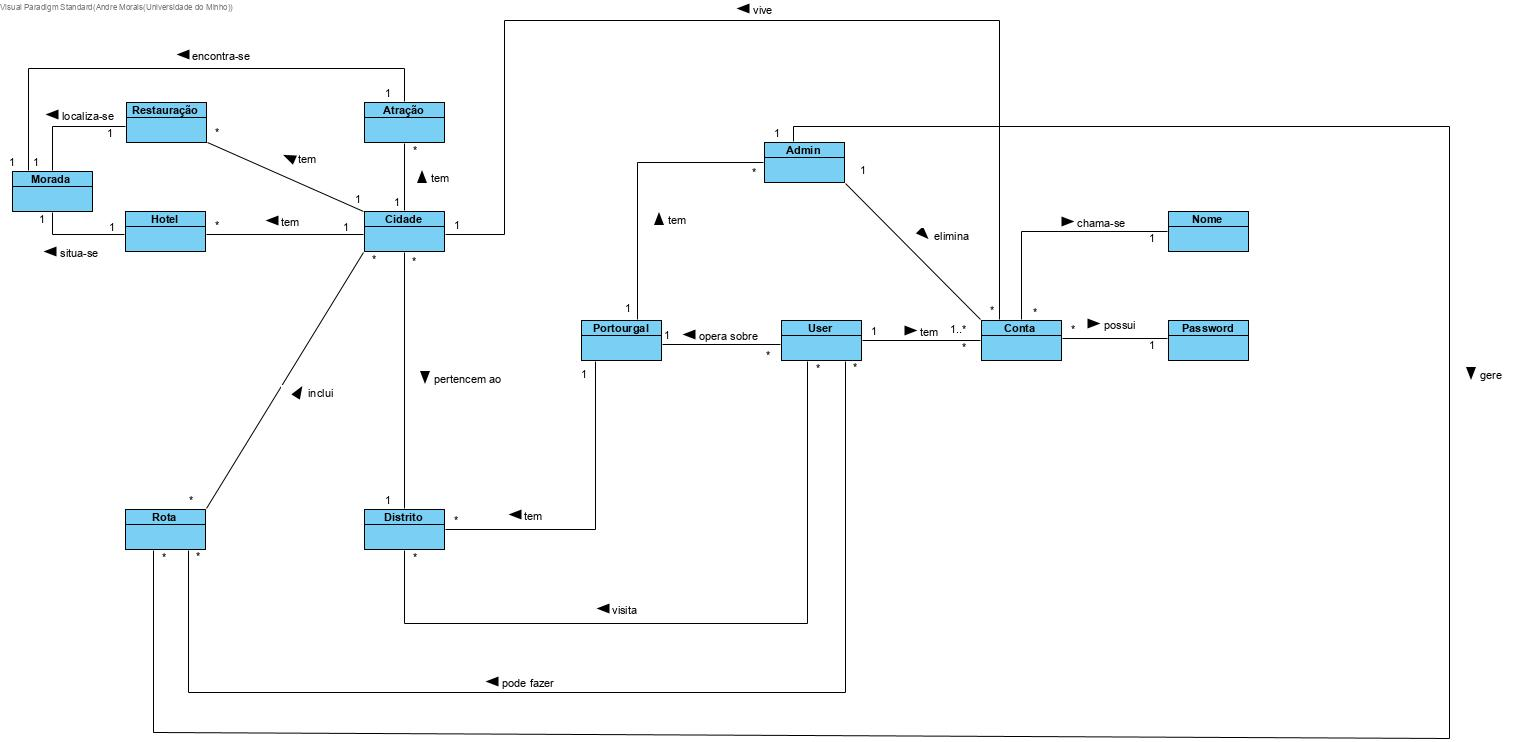
\includegraphics[width=0.9\linewidth]{images/modelodominio.jpg}
\caption{Modelo de Domínio}
\label{fig:mdominio}
\end{figure}

Consequentemente esboçamos a nossa versão, onde consideramos que as principais entidades do nosso sistema seriam: PORTOURGAL, User, Admin, Conta, Password, Nome, Distrito, Rota, Cidade, Atração, Morada, Restauração, Hotel.

Começando pelo PORTOURGAL a peça fundamental deste modelo, pois representa o “nome” da aplicação desenvolvida, que contêm Admins responsáveis pela aplicação, e para além disso é representada pelos Distritos. Os Users representam todos os utilizadores que vão operar/usar a aplicação, e estes terão uma Conta associada a cada um, com um Nome, Password e uma Cidade. Os Users operam sobre a PORTOURGAL de modo a visitar Cidades ou percorrer Rotas. As Rotas são identificadas por um conjunto de Cidades. Cada Cidade é identificada por Atrações, Restauração e Hotéis.
    
    \newpage
    
    \section{Diagrama de Use Cases}
    Os Uses Cases são uma forma sistemática de capturar requisitos funcionais, fornecendo assim uma notação diagramática que permite modelar o contexto geral do sistema. Isto é, este diagrama representa os atores do Sistema (quem utiliza o Sistema), os use cases (o que se pode fazer no Sistema) e as associações entre os atores e os use cases. As entidades que consideramos serem as principais no sistema, isto é, as entidades que efetivamente vão interagir com ele são as seguintes: User e Admin. 

O primeiro ator que identificamos foi o Administrador, que é responsável pela gestão das contas, sendo esta gestão apenas representada por um use case: Eliminar Conta. Este também é responsável por Gerir Rotas. Para isto tem que se autenticar.

O ator que se segue é o Utilizador, e este tem acesso a tudo o que a aplicação fornece, e precisa de fazer login para se autenticar. 

Inicialmente consideramos o seguinte diagrama Use Cases:

\begin{figure}[H]
\centering
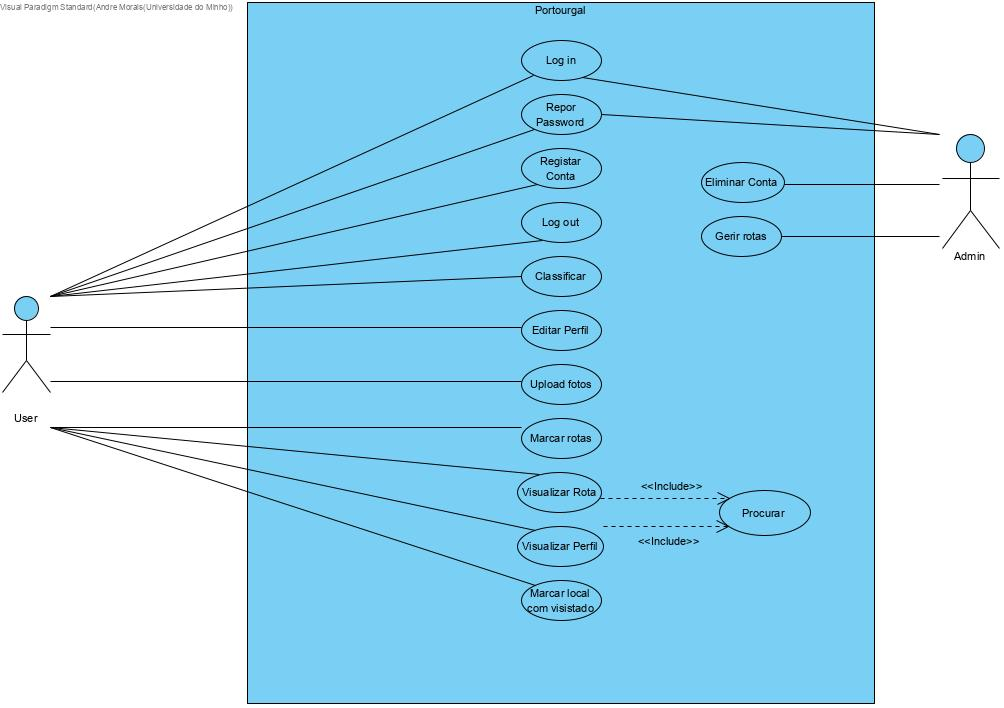
\includegraphics[width=0.9\linewidth]{images/usecases.jpg}
\caption{Diagrama de Use Cases inicial}
\label{fig:uc}
\end{figure}


\newpage

Depois de uma nova e mais profunda análise aos requisitos funcionais do sistema e aos Mockups desenvolvidos, decidimos que alguns Use Cases não iriam ser representados, portanto fomos removendo esses Use Cases do nosso diagrama. Removemos os use cases relativos à Search Bar, pois não seria necessário dado a nossa implementação do Front End da aplicação, isto é, a nível de apresentação da aplicação não iria ser necessário esta funcionalidade. O use case Upload de fotos poderia quebrar regras de segurança da aplicação, e teríamos que implementar um sistema de verificação de fotos, portanto decidimos, após uma conversa com o docente da U.C, retirar este use case. 

\begin{figure}[H]
\centering
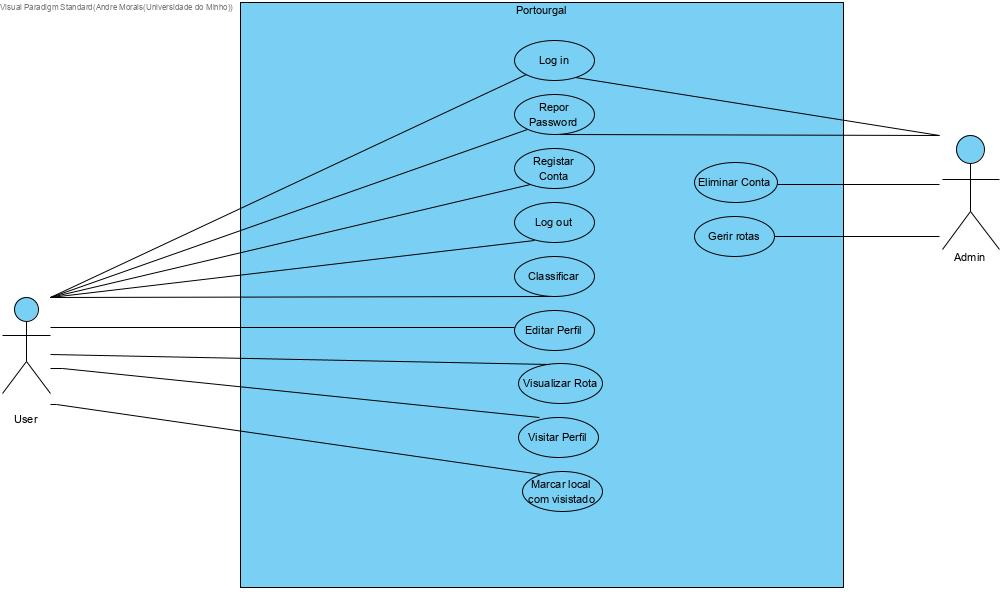
\includegraphics[width=0.9\linewidth]{images/usecases2.jpg}
\caption{Diagrama de Use Cases Final}
\label{fig:uc2}
\end{figure}

    
    \newpage
    
    \section{Especificação Use Cases}
    
    Todos os Use Case necessitam dos seus determinados fluxos, estando estes apresentados abaixo.
    
    \subsection{Criar Conta/Registar Conta}
    \textbf{Descrição:}  Consiste no ato de criar conta, em que o utilizador insere os seus dados para criar a conta associada a ele.

\textbf{Pré-condição:} A aplicação está a funcionar.

\textbf{Pós-condição:} O Sistema regista o novo User.


\textbf{Fluxo Normal:}

1. Utilizador insere as suas credencias.

2. Sistema verifica se os campos estão vazios.

3. Sistema verifica se já existe email.

4. Sistema atualiza e regista novo utilizador.

\textbf{Fluxo Alternativo: [Campos vazios]} (passo 2)

2.1 Sistema informa que os campos estão vazios.

2.2 Utilizador insere dados nos campos vazios.

2.3 Volta passo 2.


\textbf{Fluxo Alternativo: [Email já existe]} (passo 3)

3.1 Sistema informa que já existe o email inserido.

3.2 Utilizador insere novo email.

3.3 Volta passo 3.
    
    \subsection{Visualizar Perfil}
    \textbf{Descrição:} Utilizador visita perfil de outros utilizadores

\textbf{Pré-condição:} Utilizador está autenticado.

\textbf{Pós-condição:} Utilizador visita perfil de outro utilizador.

\textbf{Fluxo Normal:}

1. Utilizador carrega na página ScoreBoard.

2. Sistema carrega ScoreBoard.

3. Utilizador carrega na foto do Utilizador que pretende visitar.

4. Sistema carrega perfil do utilizador a visitar.
    
    \newpage
    
    \subsection{Login}
    \textbf{Descrição:}  Consiste em se autenticar na aplicação PORTOURGAL.

\textbf{Pré-condição:} A aplicação está a funcionar.

\textbf{Pós-condição:} Utilizador está autenticado.

\textbf{Fluxo Normal:}

1. Sistema pede credenciais ao utilizador.

2. Utilizador insere email e palavra passe.

3. Sistema verifica credenciais inseridas.

4. Utilizador autentica-se.

\textbf{Fluxo Alternativo: [Credenciais erradas]} (passo 3)

3.1 Sistema informa que as credenciais estão erradas.

3.2 Volta para o passo 1.
    
    \subsection{Logout}
    \textbf{Descrição:}  Consiste em se desconectar da aplicação PORTOURGAL.

\textbf{Pré-condição:} Utilizador/Admin está autenticado.

\textbf{Pós-condição:} Utilizador/Admin deixa de estar autenticado.

\textbf{FLuxo Normal:}

1. Utilizador escolhe fazer logout.

2. Sistema informa que o utilizador está agora desconectado.
    
    \subsection{Repor Password}
    \textbf{Descrição:}  Consiste no ato de repor a palavra passe do User.

\textbf{Pré-condição:} O utilizador está autenticado.

\textbf{Pós-condição:} O utilizador tem nova password..

\textbf{FLuxo Normal:}

1. Utilizador escolhe editar o perfil.

2. Utilizador insere nova palavra passe.

3. Sistema atualiza e associa nova palavra passe.
    
    \newpage
    
    
    \subsection{Classificar Atração}
    \textbf{Descrição:} Consiste no ato do User classificar uma Atração.

\textbf{Pré-condição:} O utilizador está autenticado.

\textbf{Pós-condição:} Sistema adquire nova classificação de uma atração.

\textbf{Fluxo Normal:}

1. Utilizador procura Atração que pretende classificar.

2. Utilizador escolhe classificação a atribuir.

3. Sistema atualiza com nova classificação inserida.
    
    \subsection{Editar Perfil}
    \textbf{Descrição:} Consiste no ato de editar credenciais de um User.

\textbf{Pré-condição:} O utilizador está autenticado.

\textbf{Pós-condição:} O utilizador tem lhe associado novas credenciais.

\textbf{Fluxo Normal:}

1. Utilizador escolhe editar o perfil.

2. Utilizador insere novas credenciais que pretende mudar.

3. Sistema verifica se User mudou email.

4. Sistema verifica se já existe email.

5. Sistema atualiza com as novas credenciais.


\textbf{Fluxo Alternativo: [Email já existe]} (passo 4)

4.1 Sistema informa que já existe o email inserido.

4.2 Volta passo 2.


\subsection{Visualizar Rota}

\textbf{Descrição:} Consiste no ato do User visualizar uma Rota do Sistema.

\textbf{Pré-condição:} O utilizador está autenticado.

\textbf{Pós-condição:} Sistema mostra rota procurada. 

\textbf{Fluxo Normal:}

1. Utilizador procura Rota que pretende visualizar.

2. Sistema mostra Rota.
    
    \newpage
    
    
    \subsection{Marcar local como visitado}
    \begin{enumerate}
    \item Definição Requisitos de utilizador
    \begin{itemize}
        \item O utilizador pode marcar uma atracão como visitado.
    \end{itemize}
    \item Especificação de requisitos de sistema
    \begin{itemize}
        \item O sistema atualiza o switch para on se esta tivesse em off;
        \item O sistema adiciona a foto da atração ao perfil se o botão estiver em on;
        \item O sistema atualiza o switch para off se esta tivesse em on;
        \item O sistema remove a foto da atração do perfil se o botão estiver em off.
    \end{itemize}
\end{enumerate}
    
    \subsection{Remover Conta}
    \textbf{Descrição:} Administrador remove conta existente de um user.

\textbf{Pré-condição:} Administrador está autenticado.

\textbf{Pós-condição:} Sistema remove conta do Utilizador. 

\textbf{Fluxo Normal:}	

1. Administrador insere email do Utilizador.

2. Sistema verifica se existe o email.

3. Sistema atualiza e remove o Utiliador.

\textbf{Fluxo Alternativo: [Email já existe]} (passo 2)

2.1 Sistema informa que conta já não existe.
    
    \subsection{Gerir Rotas}
    \textbf{Descrição:} Administrador gere rotas do Sistema.

\textbf{Pré-condição:} Administrador está autenticado.

\textbf{Pós-condição:} Sistema atualiza com novas rotas.

\textbf{Fluxo Normal:}

1. Administrador adiciona ou remove rota.

2. Sistema atualiza.
    
    \section{Diagrama de Classes}
    Decidimos implementar um Diagrama de Classes pois são diagramas estruturais que permitem ilustrar as classes e o relacionamento entre as mesmas. Assim, estes permitem descrever a estrutura de um sistema, modelando ainda os atributos e as operações entre objetos. \par Nesse sentido, a obtenção deste diagrama resultou de uma análise cuidada do modelo de domínio, identificando assim, quais as classes suscetíveis de serem criadas.

\begin{figure}[H]
\centering
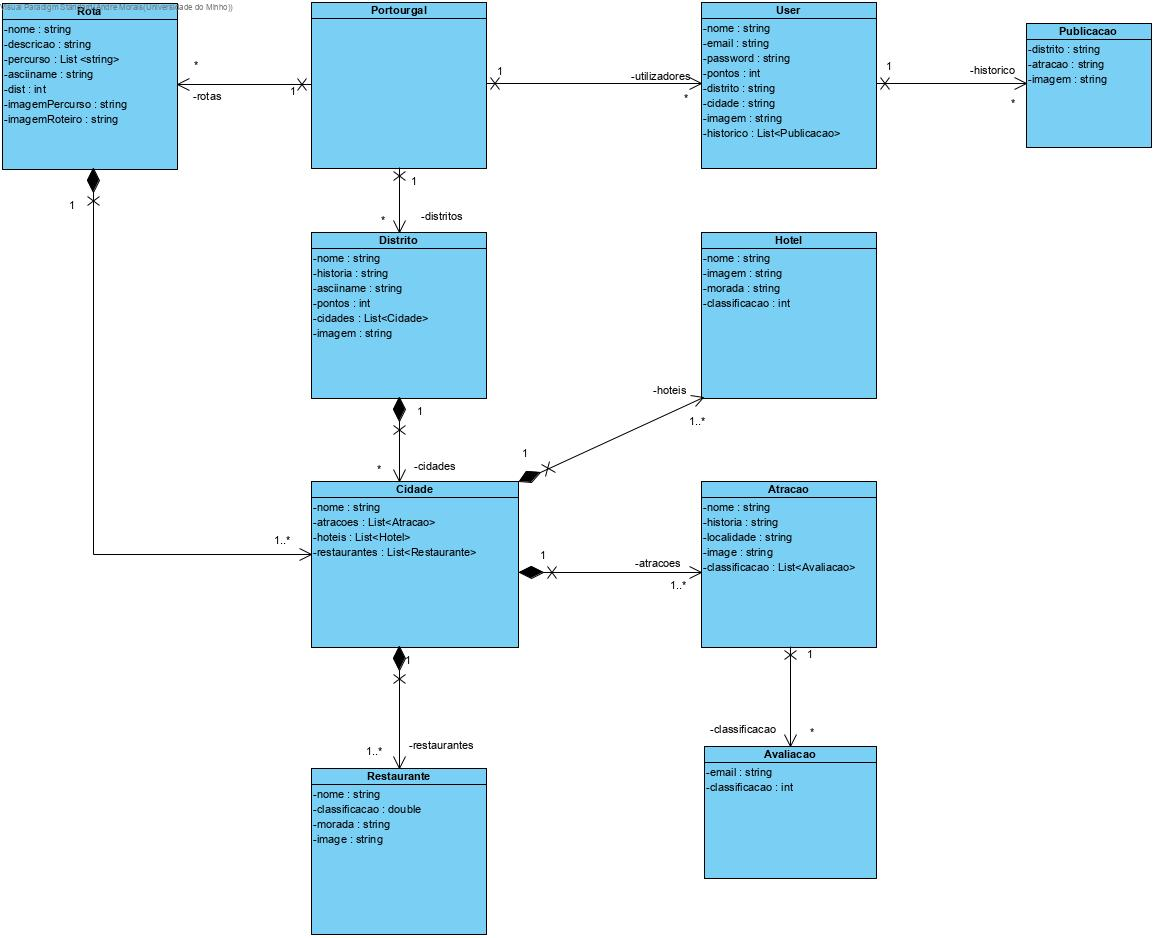
\includegraphics[width=0.9\linewidth]{images/diagrama_classe.jpg}
\caption{Diagrama de classes.}
\end{figure}

\newpage
	% CHAPTER - Application -------------------------
	\chapter{Implementação}
    
    \section{Funcionalidades}
    \subsection{Página Inicial}
    \begin{figure}[H]
\centering
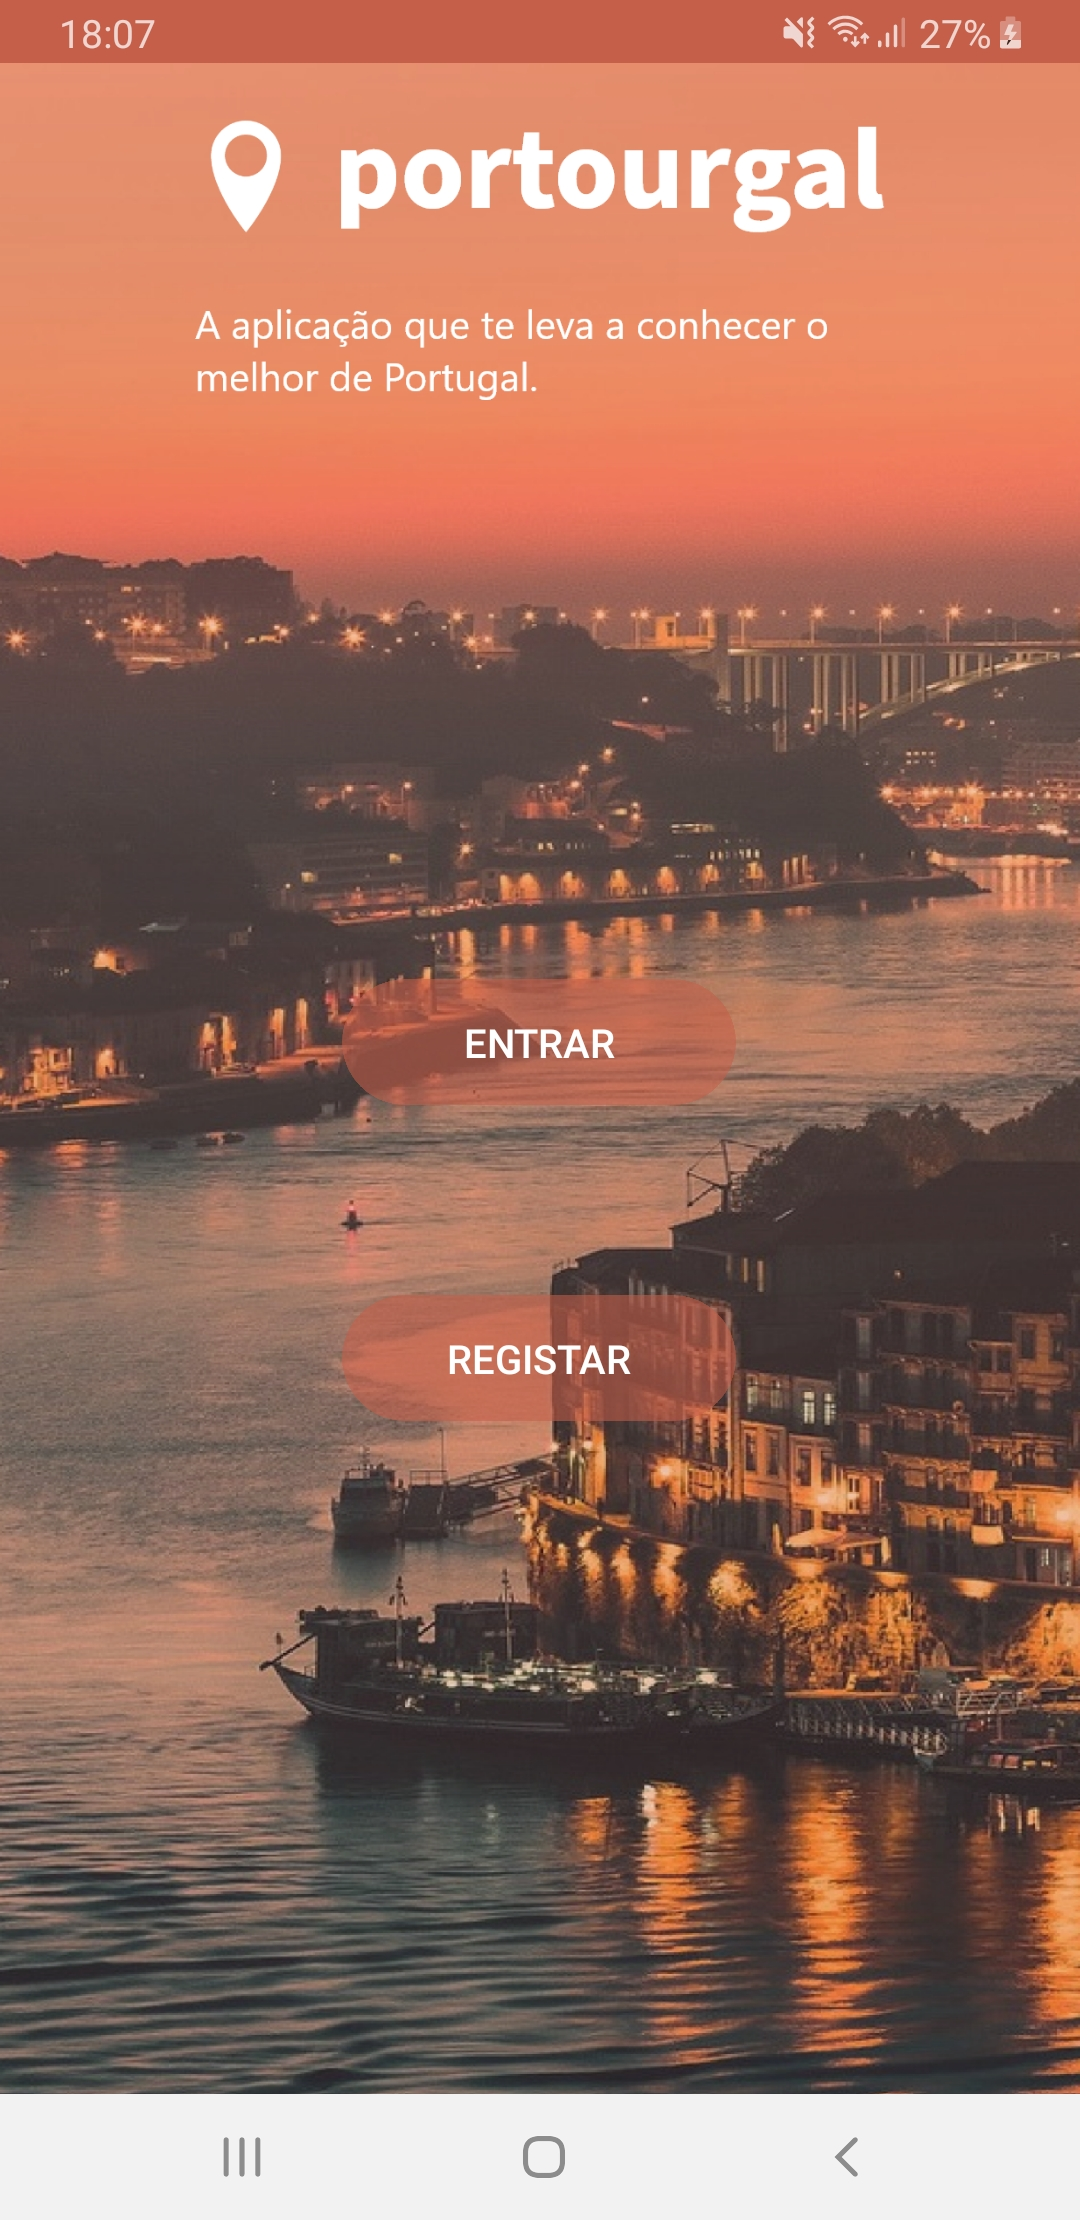
\includegraphics[width=0.3\linewidth]{images/inicio.jpg}
\caption{Página inicial.}
\end{figure}

Esta é a página inicial da aplicação, sendo esta apresentada sempre que o utilizador queira utilizar a aplicação.
    
    \newpage
    
    \subsection{Login}
    \begin{figure}[H]
\centering
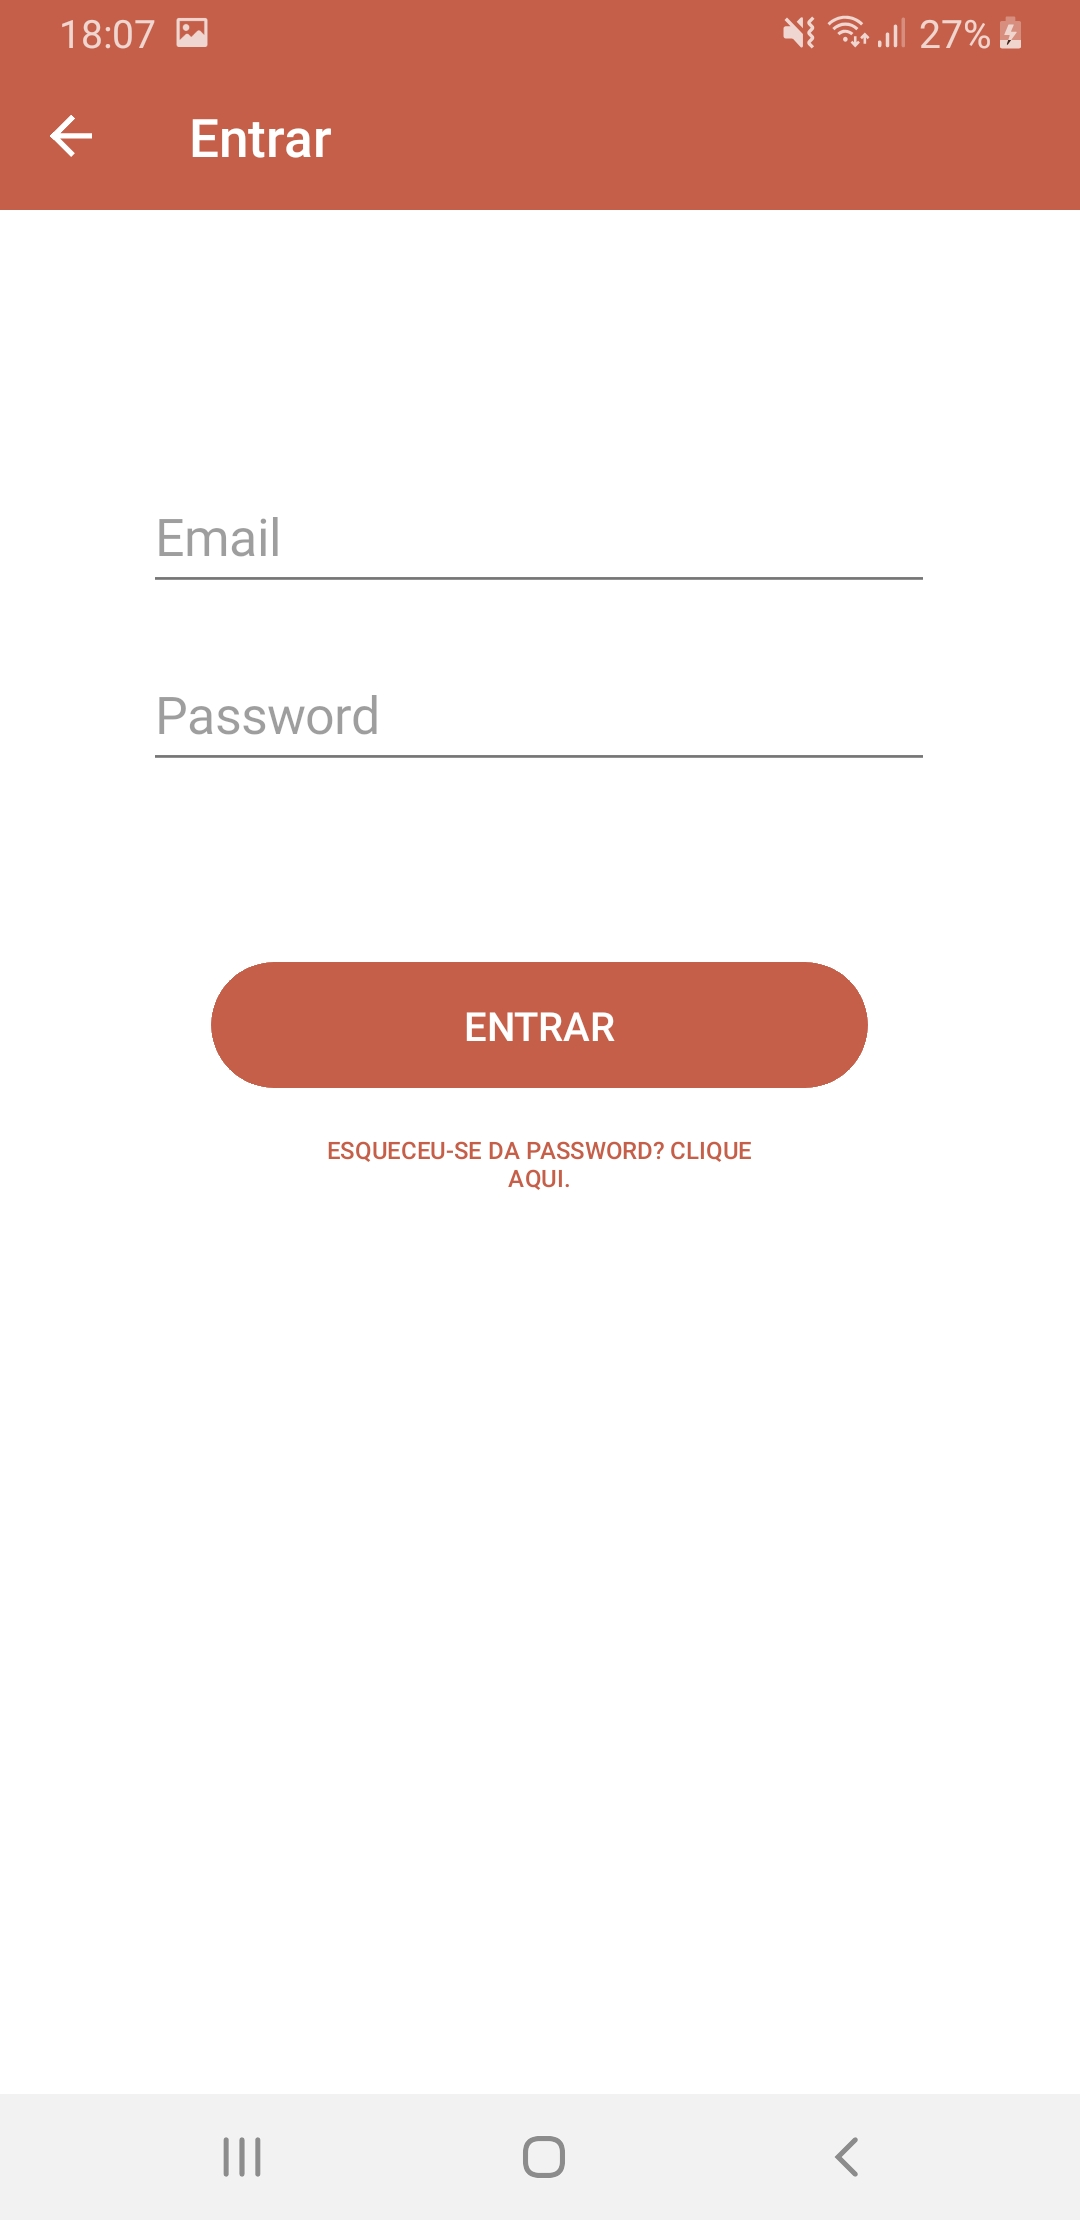
\includegraphics[width=0.5\linewidth]{images/entrar.jpg}
\caption{Página de login.}
\end{figure}
    
    \newpage
    
    \subsection{Registar}
    \begin{figure}[H]
\centering
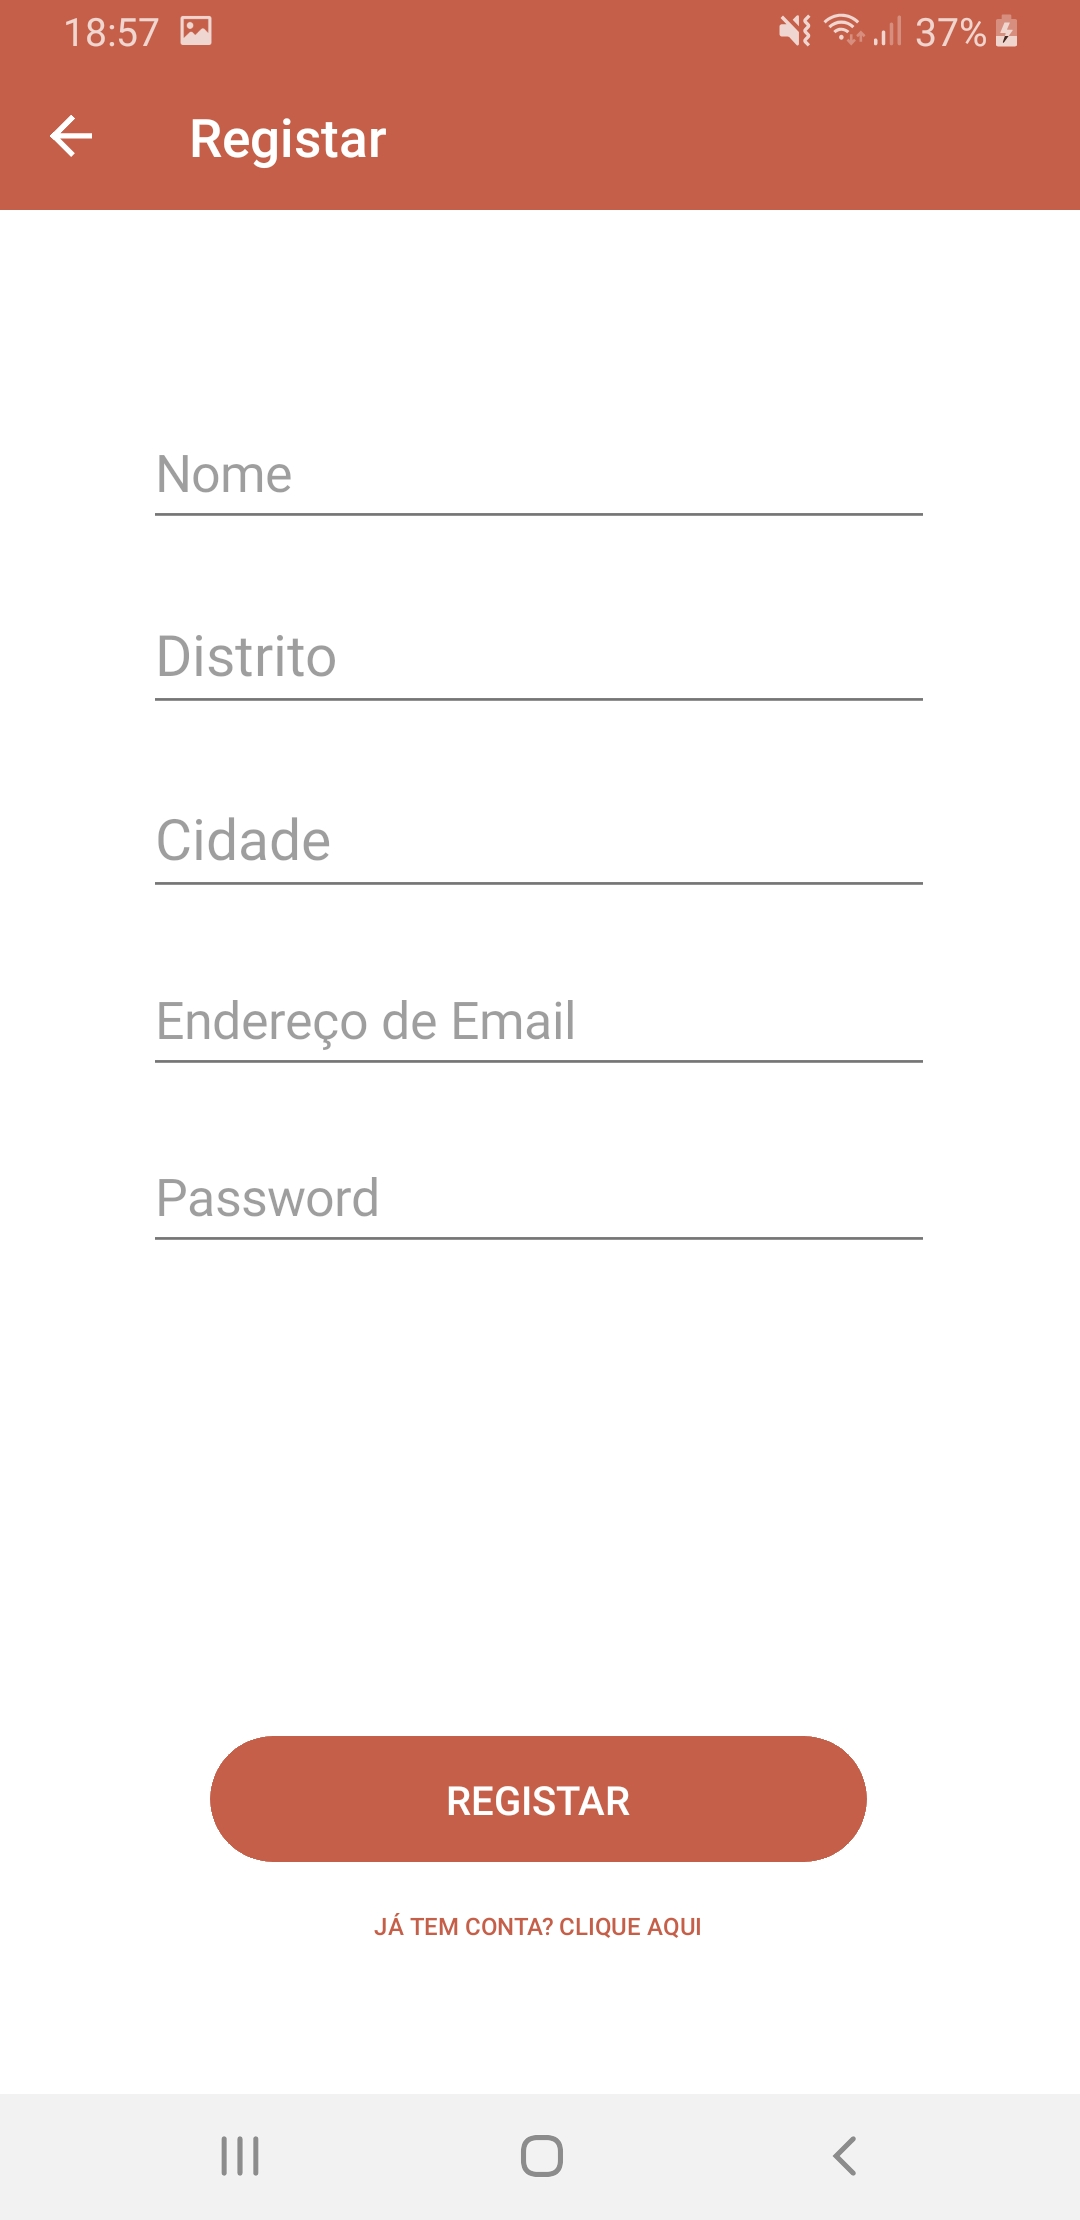
\includegraphics[width=0.5\linewidth]{images/registar.jpg}
\caption{Página de registo}
\end{figure}
    
    \newpage
    
    \subsection{Perfil de utilizador}
    \begin{figure}[H]
\centering
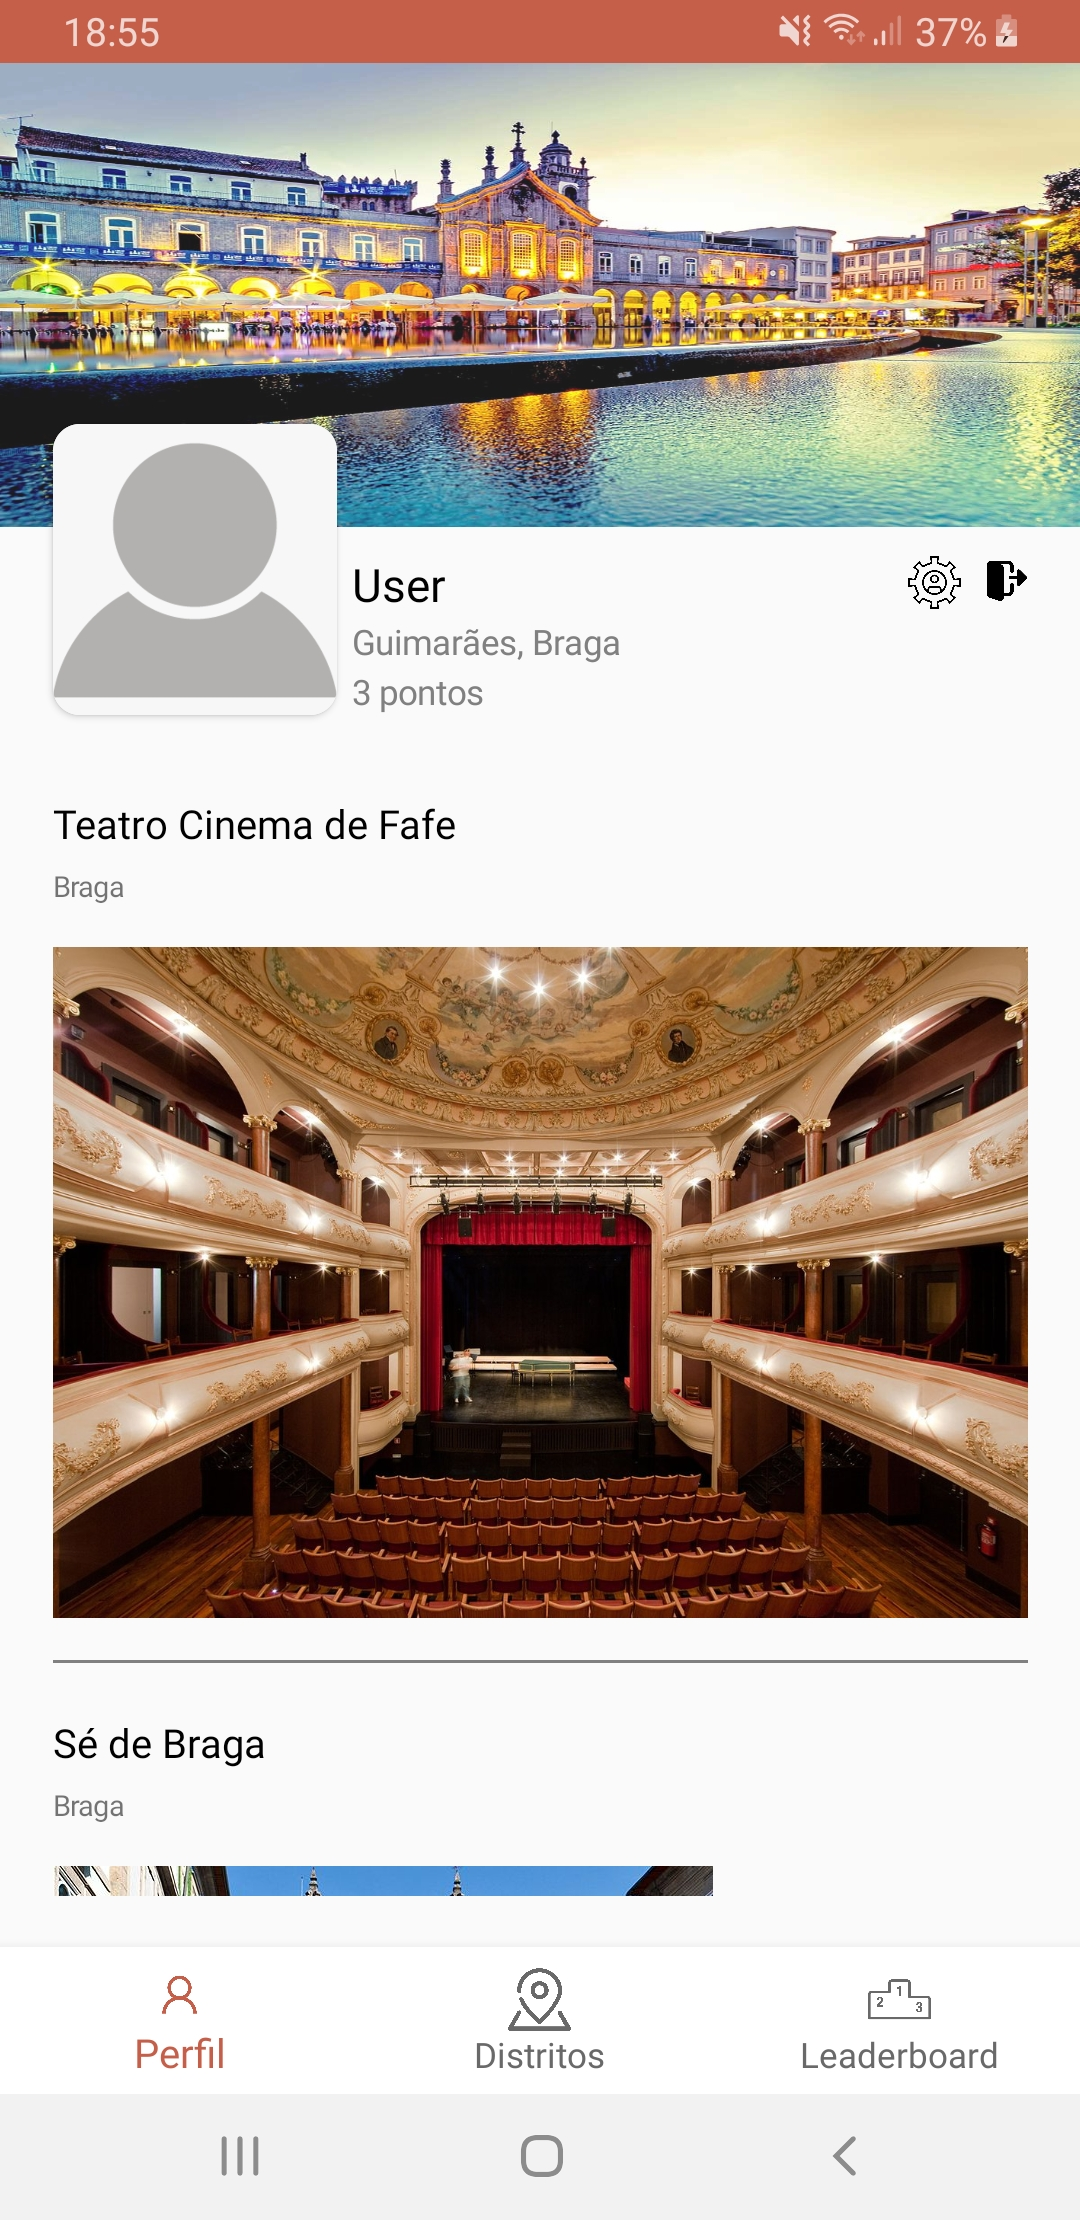
\includegraphics[width=0.5\linewidth]{images/perfilUtilizador.jpg}
\caption{Página de perfil}
\end{figure}
    
    \newpage
    
    \subsection{Editar perfil}
    \textbf{Descrição:} Consiste no ato de editar credenciais de um User.

\textbf{Pré-condição:} O utilizador está autenticado.

\textbf{Pós-condição:} O utilizador tem lhe associado novas credenciais.

\textbf{Fluxo Normal:}

1. Utilizador escolhe editar o perfil.

2. Utilizador insere novas credenciais que pretende mudar.

3. Sistema verifica se User mudou email.

4. Sistema verifica se já existe email.

5. Sistema atualiza com as novas credenciais.


\textbf{Fluxo Alternativo: [Email já existe]} (passo 4)

4.1 Sistema informa que já existe o email inserido.

4.2 Volta passo 2.


\subsection{Visualizar Rota}

\textbf{Descrição:} Consiste no ato do User visualizar uma Rota do Sistema.

\textbf{Pré-condição:} O utilizador está autenticado.

\textbf{Pós-condição:} Sistema mostra rota procurada. 

\textbf{Fluxo Normal:}

1. Utilizador procura Rota que pretende visualizar.

2. Sistema mostra Rota.
    
    \newpage
    
    \subsection{Upload de uma imagem}
    \begin{figure}[H]
\centering
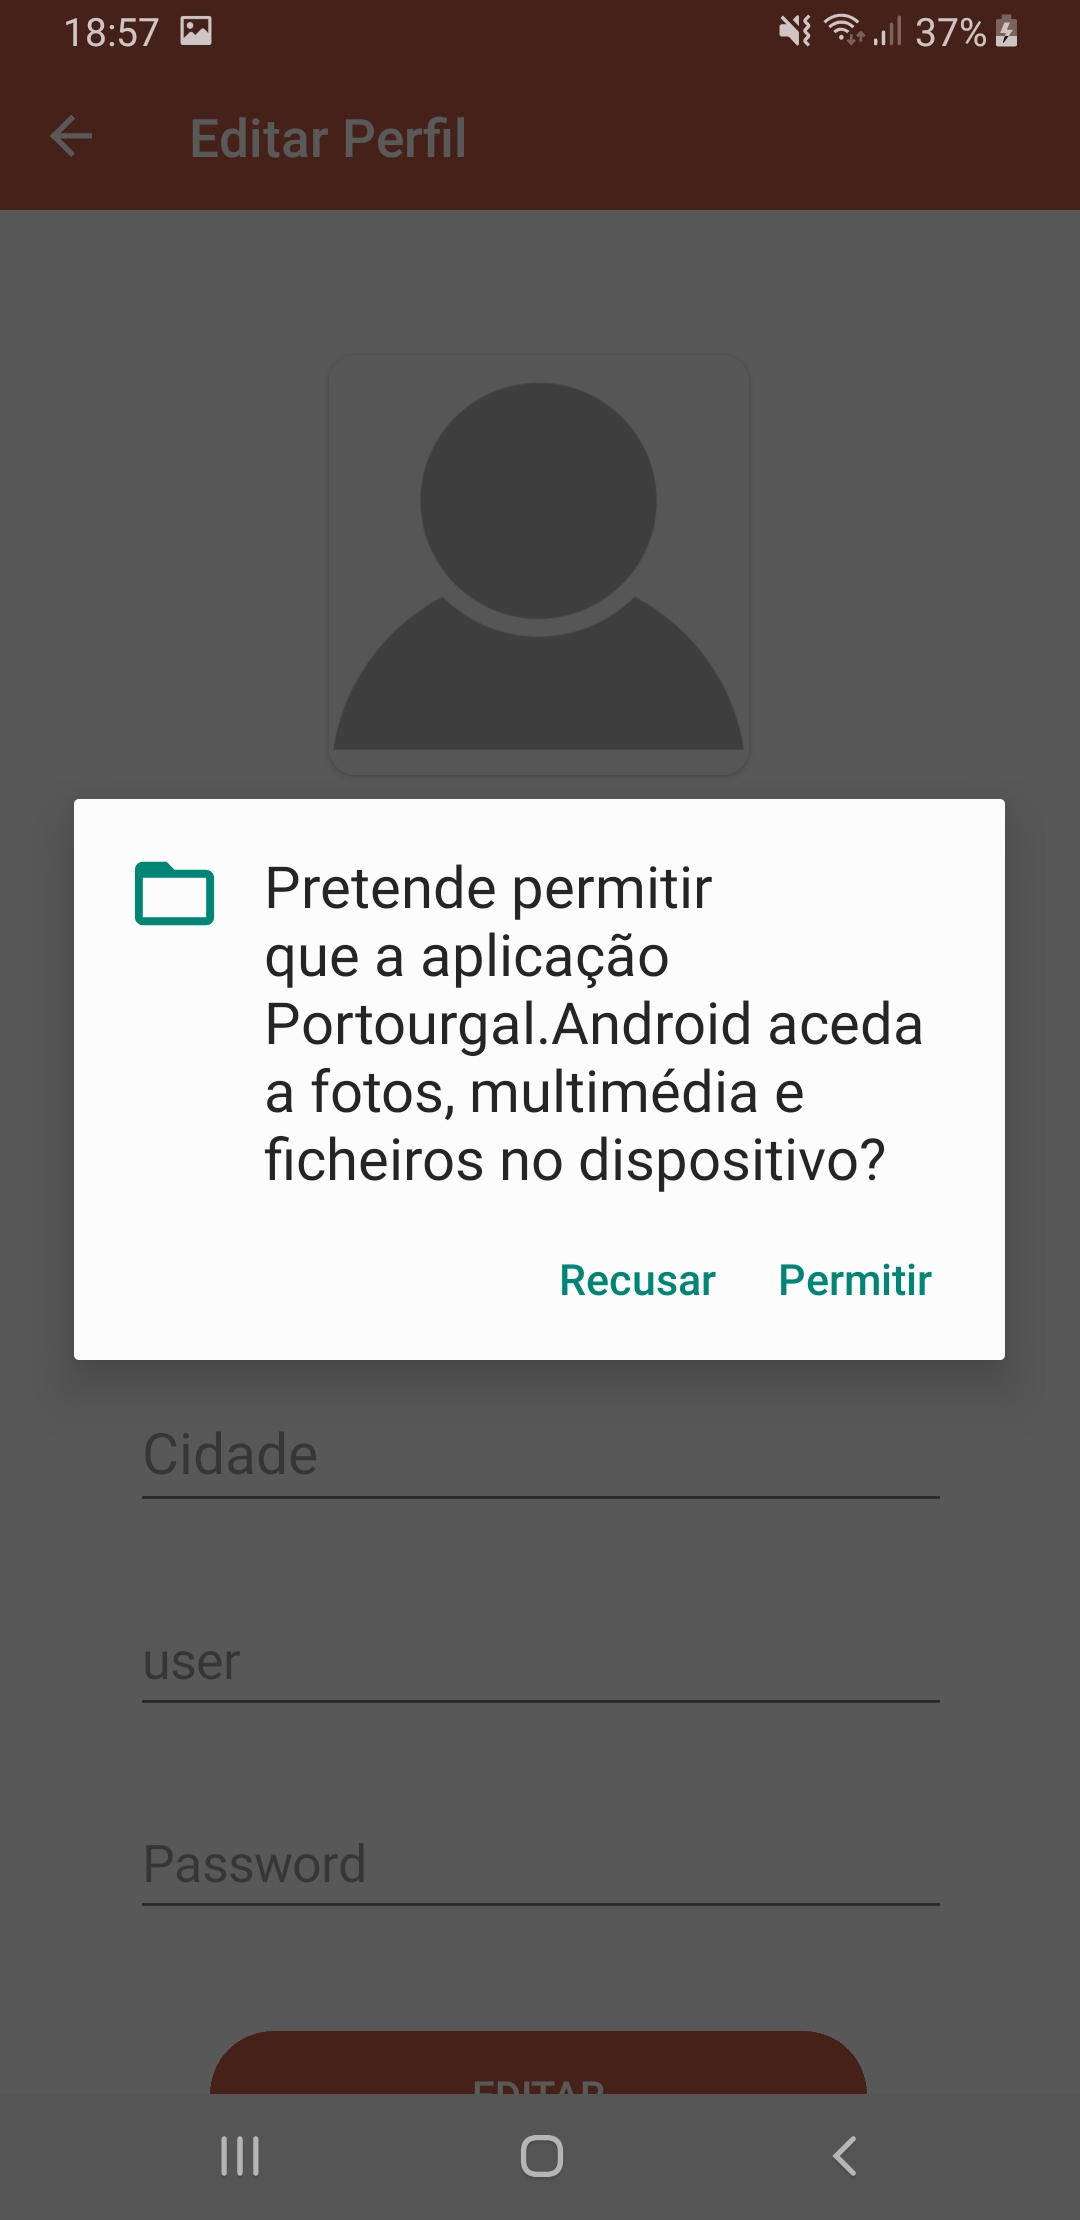
\includegraphics[width=0.5\linewidth]{images/anexarImagem.jpg}
\caption{Anexar uma imagem para foto de perfil.}
\end{figure}
    
    \newpage
    
    \subsection{Navegar pelos distritos/roteiros}
    \begin{figure}[H]
    \centering
    \begin{subfigure}{.5\textwidth}
        \centering
        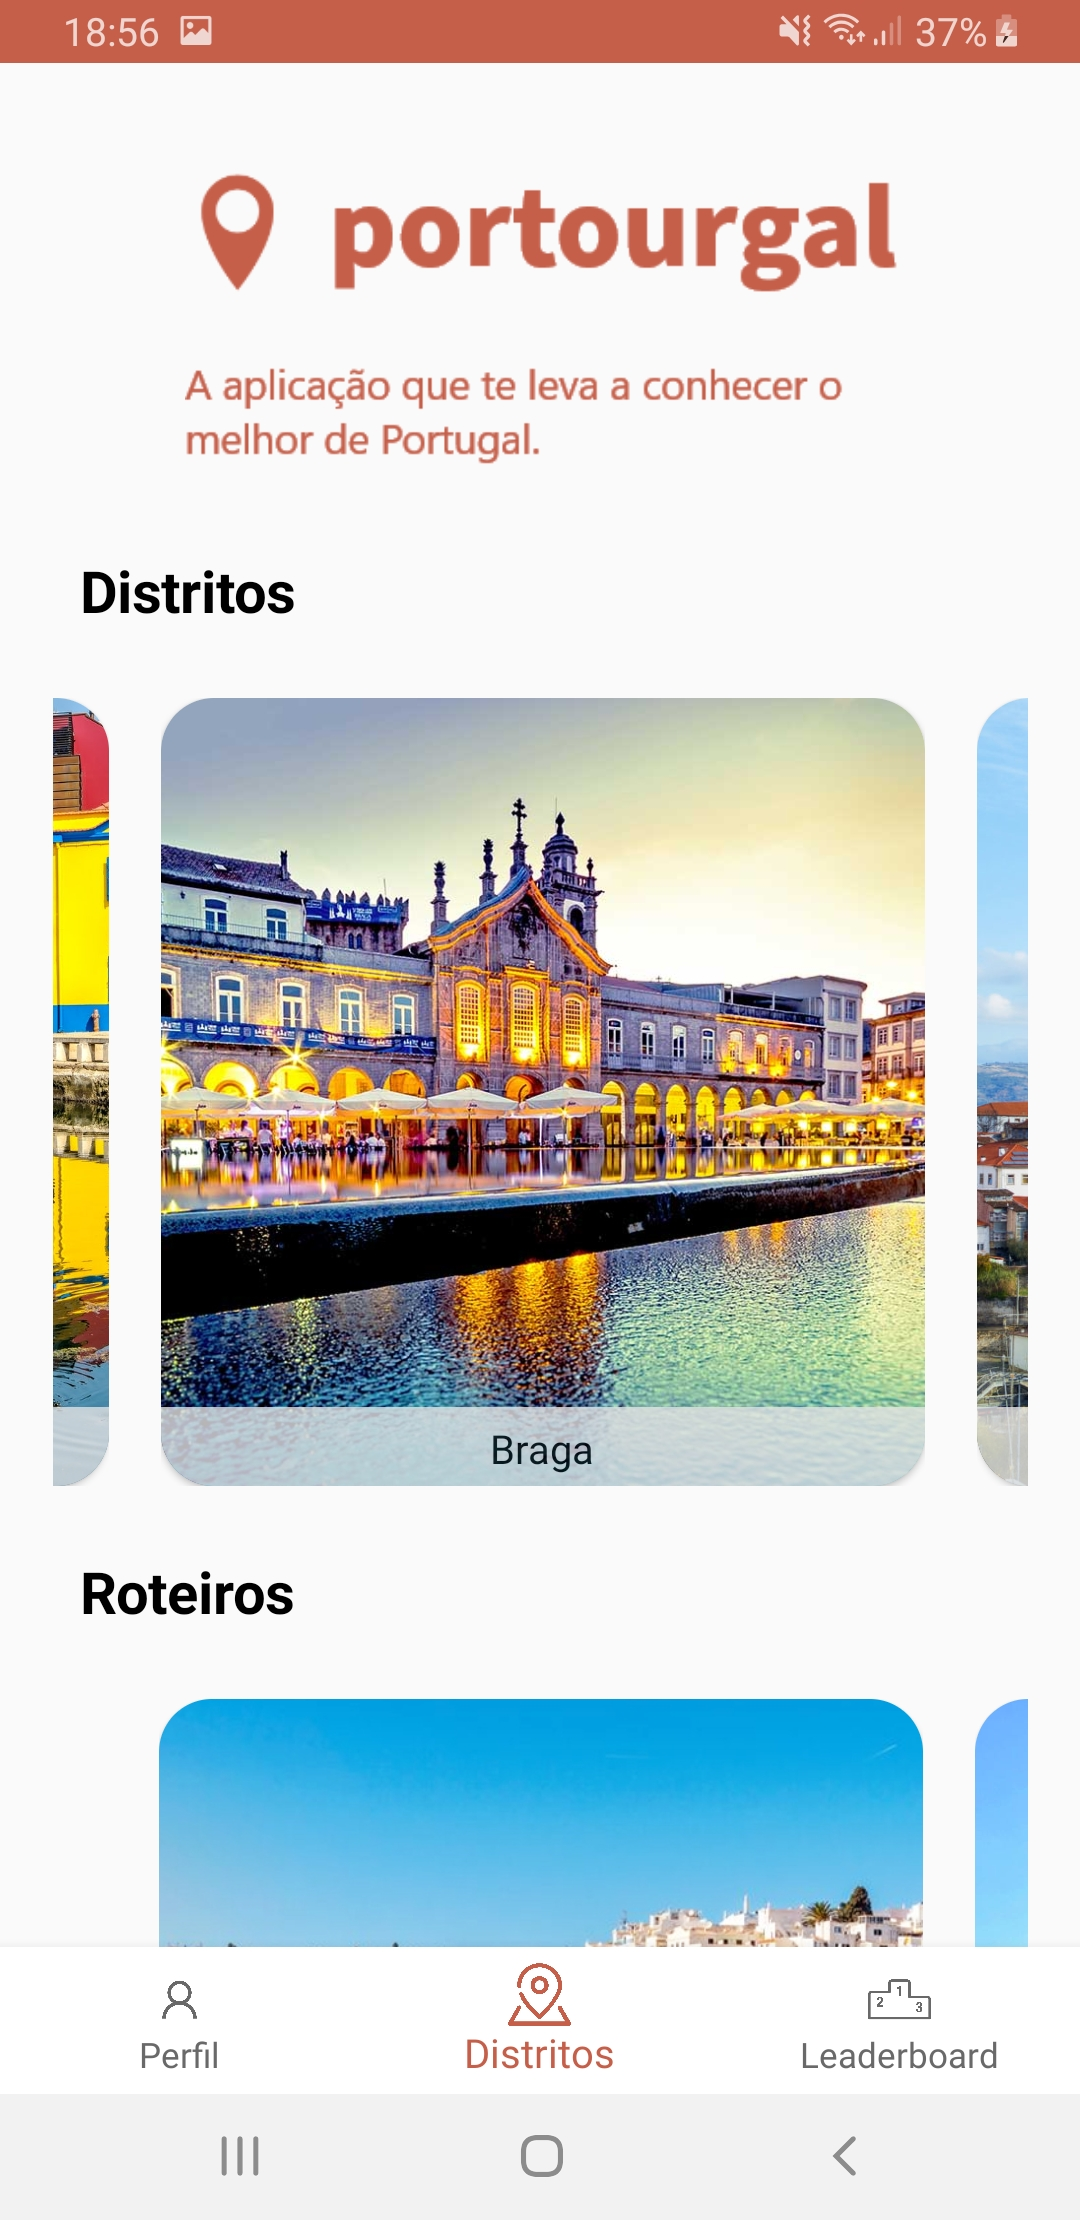
\includegraphics[width=0.9\linewidth]{images/distritos.jpg}
    \end{subfigure}%
    \begin{subfigure}{.5\textwidth}
        \centering
        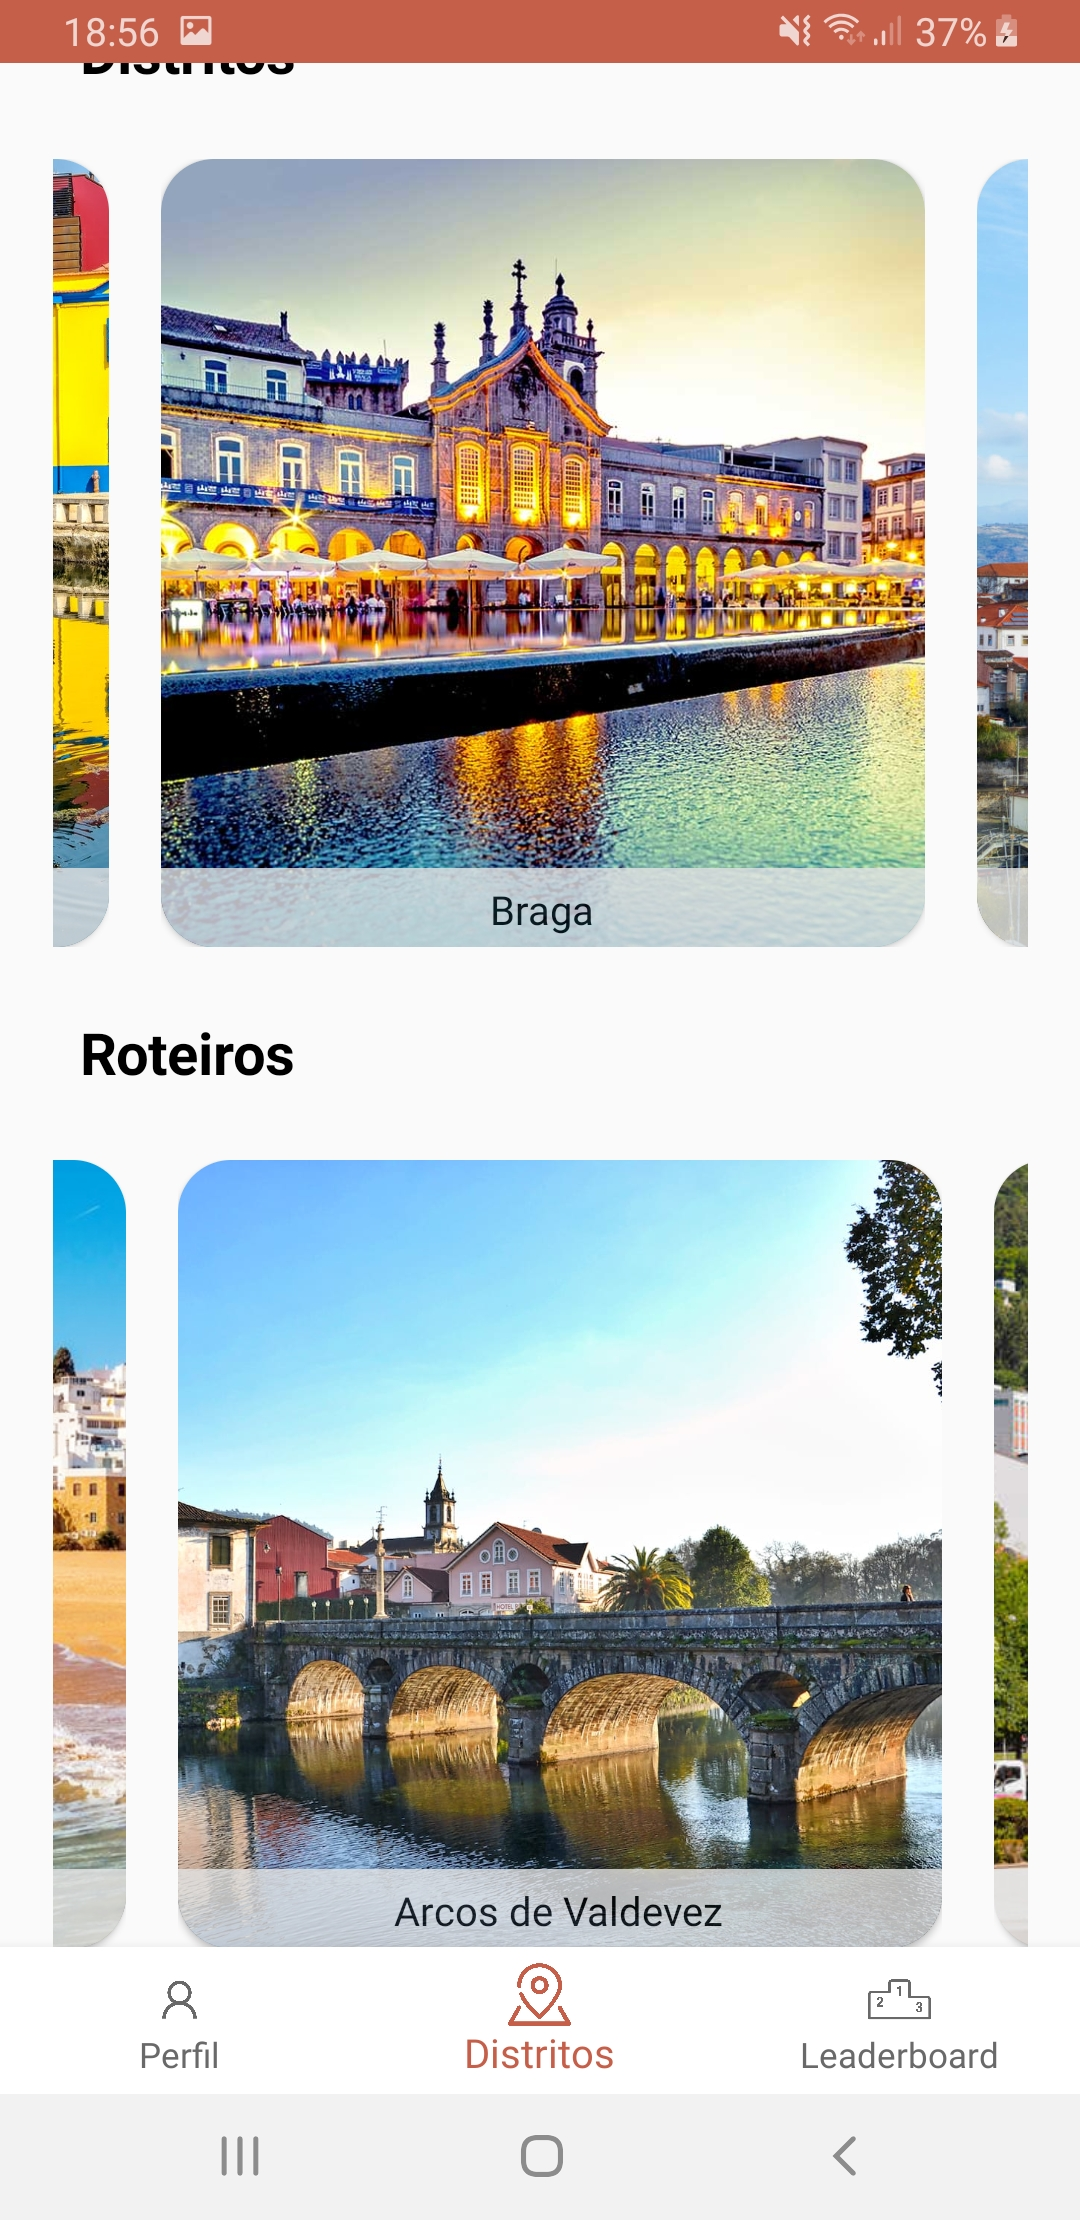
\includegraphics[width=0.9\linewidth]{images/distritos2.jpg}
    \end{subfigure}
    \caption{Página dos distritos e roteiros.}
\end{figure}
    
    \newpage
    
    \subsection{Conteúdo de um distrito}
    \begin{figure}[H]
\centering
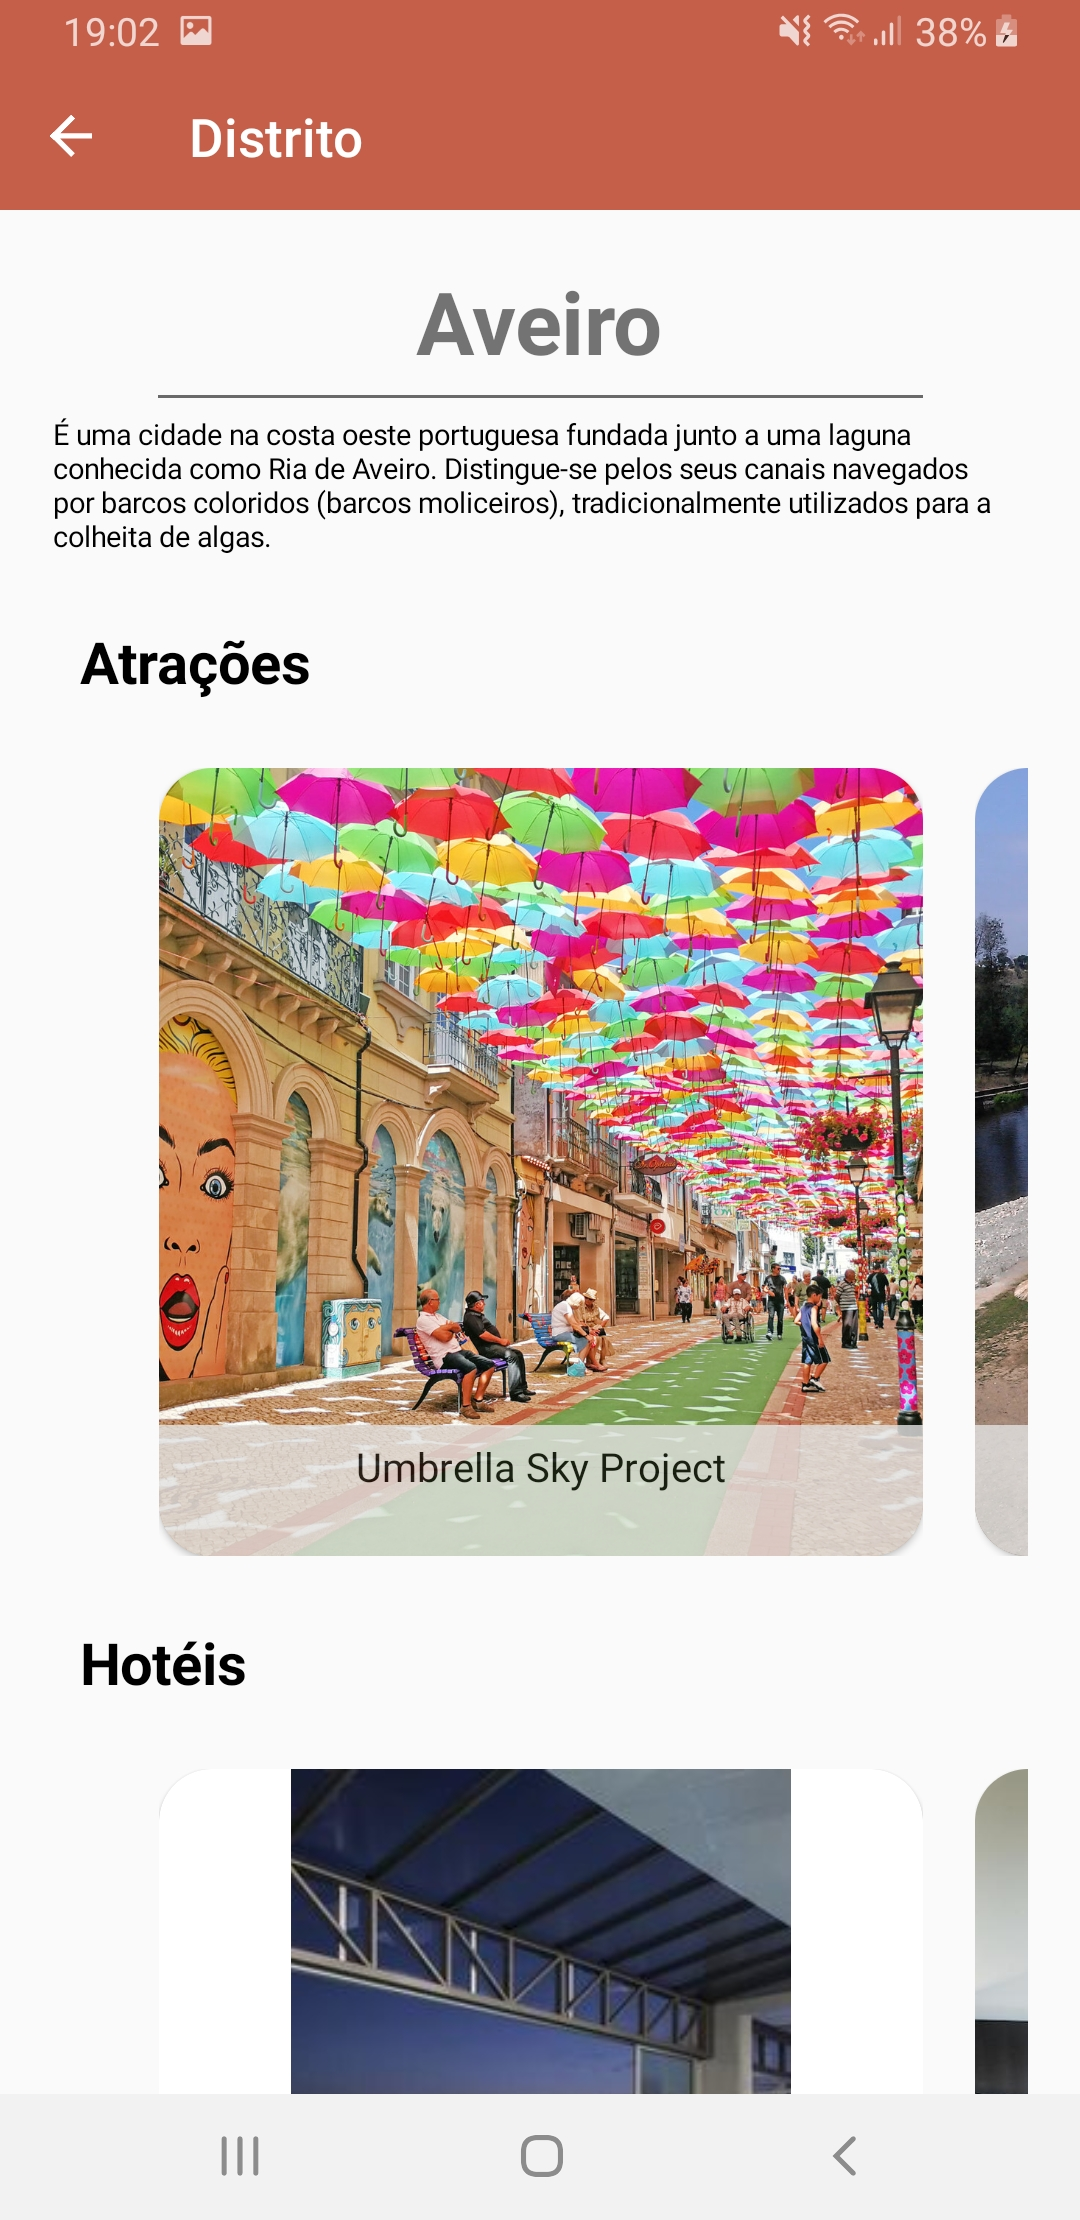
\includegraphics[width=0.5\linewidth]{images/distritosEspecifico.jpg}
\caption{Exemplo de um distrito.}
\end{figure}
    
    \newpage
    
    \subsection{Atração}
    \begin{enumerate}
    \item Definição Requisitos de utilizador
    \begin{itemize}
        \item O utilizador consegue visualizar a informação desta atração com uma pequena descrição, uma fotografia e respetiva localidade/morada;
        \item O utilizador também pode classificar e marcar como visitado.
    \end{itemize}
    \item Especificação de requisitos de sistema
    \begin{itemize}
        \item O sistema deve possuir na base de dados a informação da atração e apresentá-la no ecrã do utilizador.
    \end{itemize}
\end{enumerate}
    
    \newpage
    
    \subsection{Percurso}
    \begin{figure}[H]
\centering
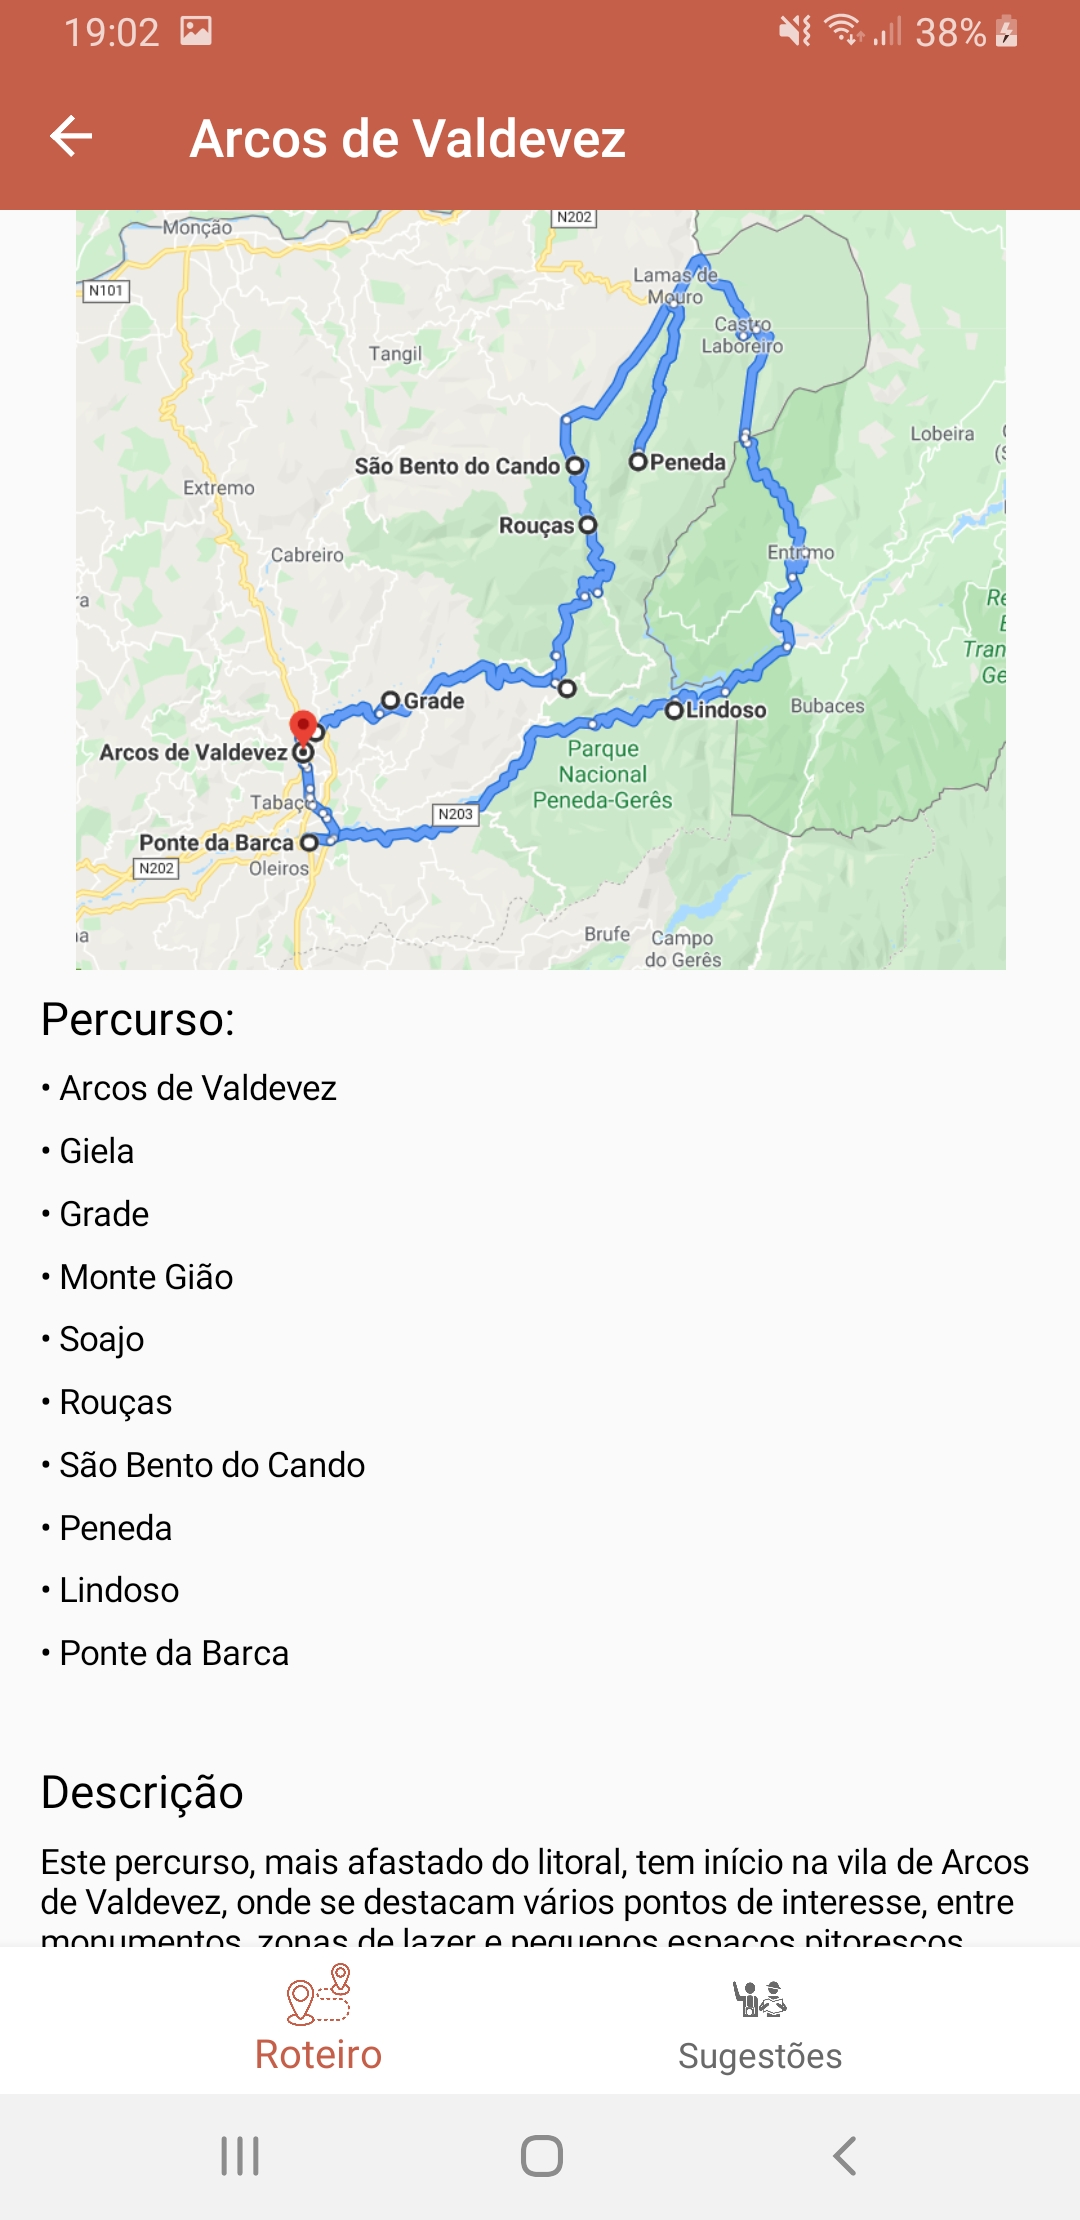
\includegraphics[width=0.5\linewidth]{images/percurso.jpg}
\caption{Exemplo de um percurso.}
\end{figure}
    
    \newpage
    
    \subsection{Sugestões para um percurso}
    \begin{figure}[H]
\centering
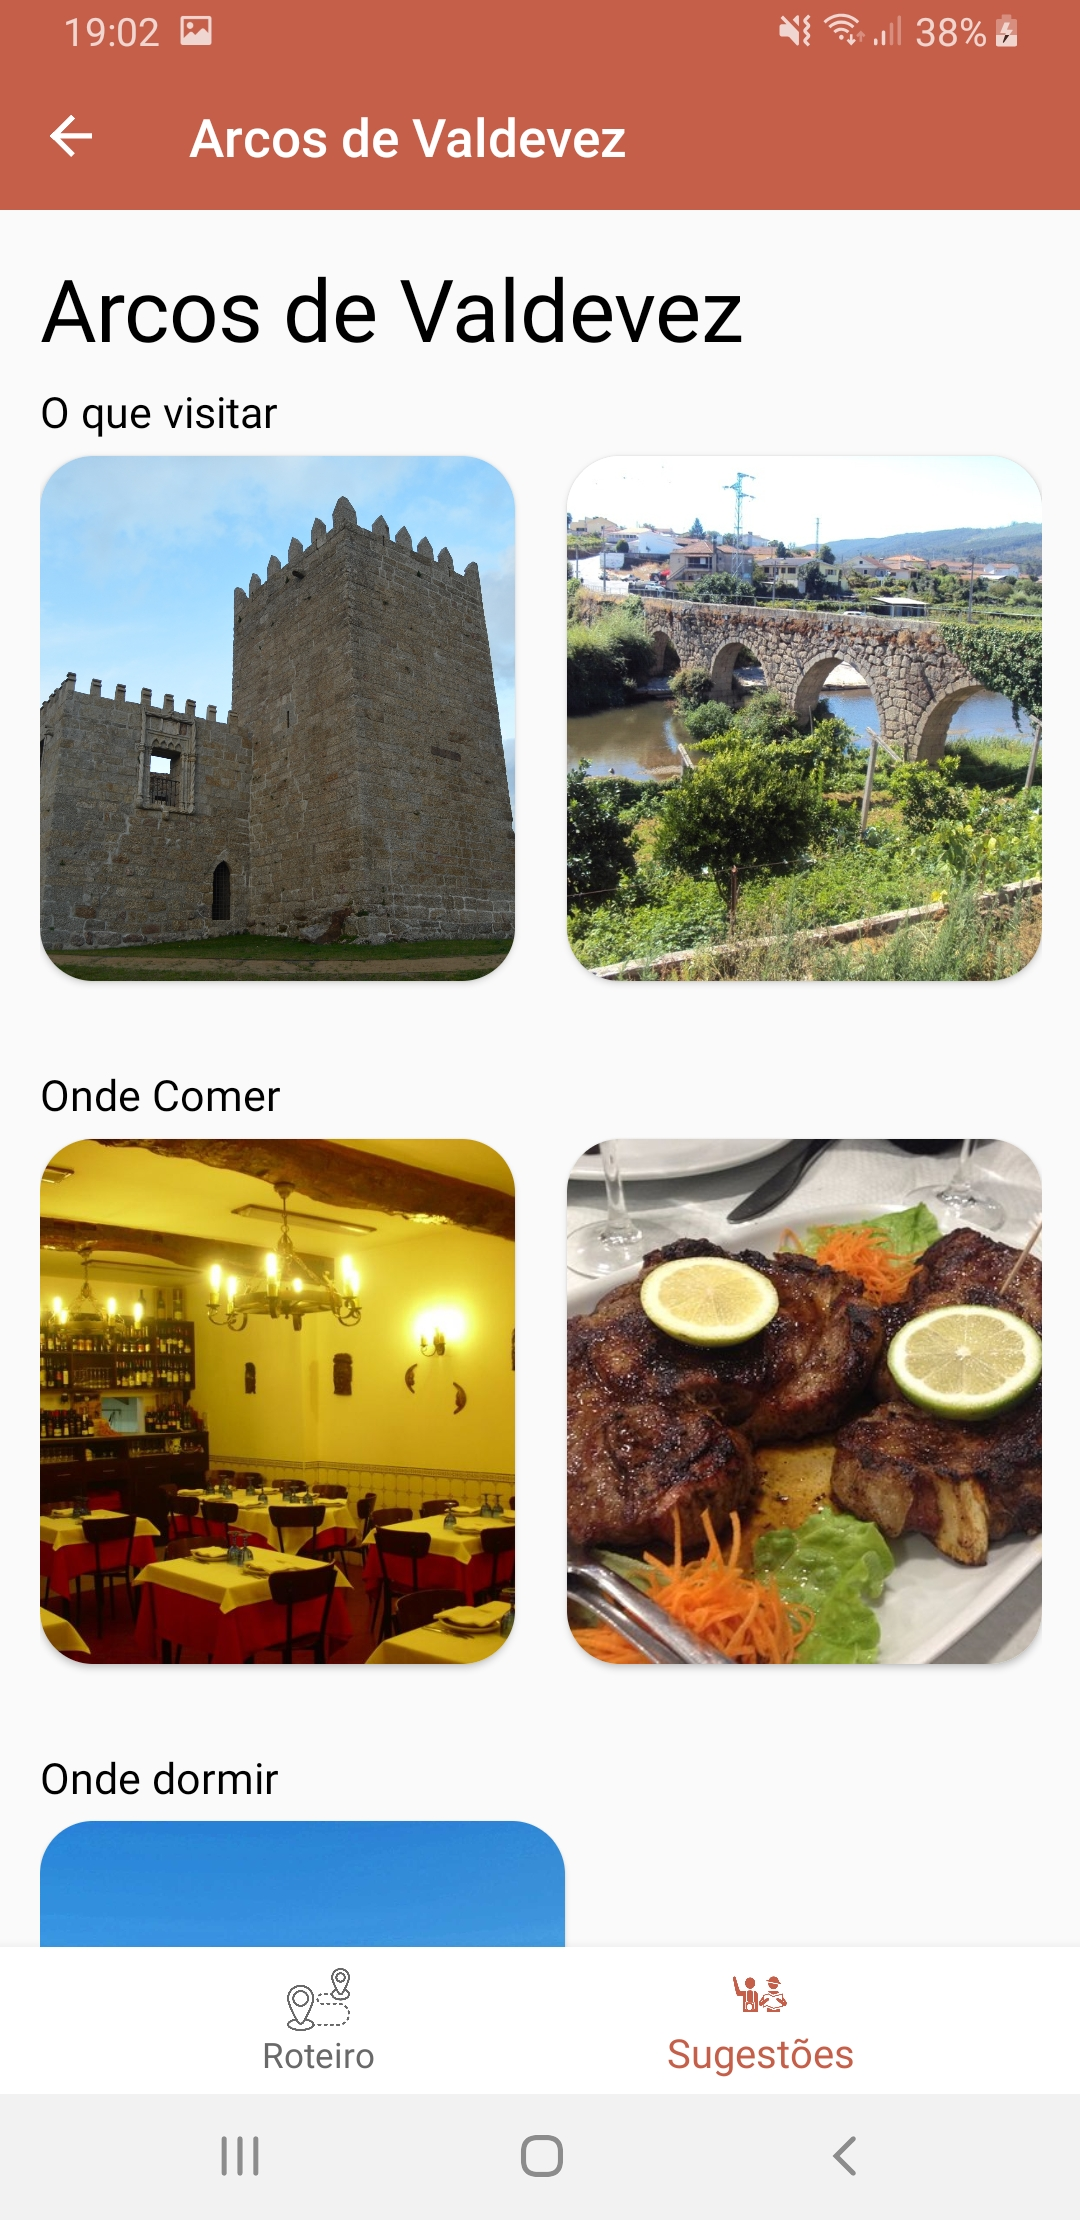
\includegraphics[width=0.5\linewidth]{images/sugestoes.jpg}
\caption{Sugestões para um percurso exemplo.}
\end{figure}
    
    \newpage
    
    \subsection{Leaderboard}
    \begin{figure}[H]
\centering
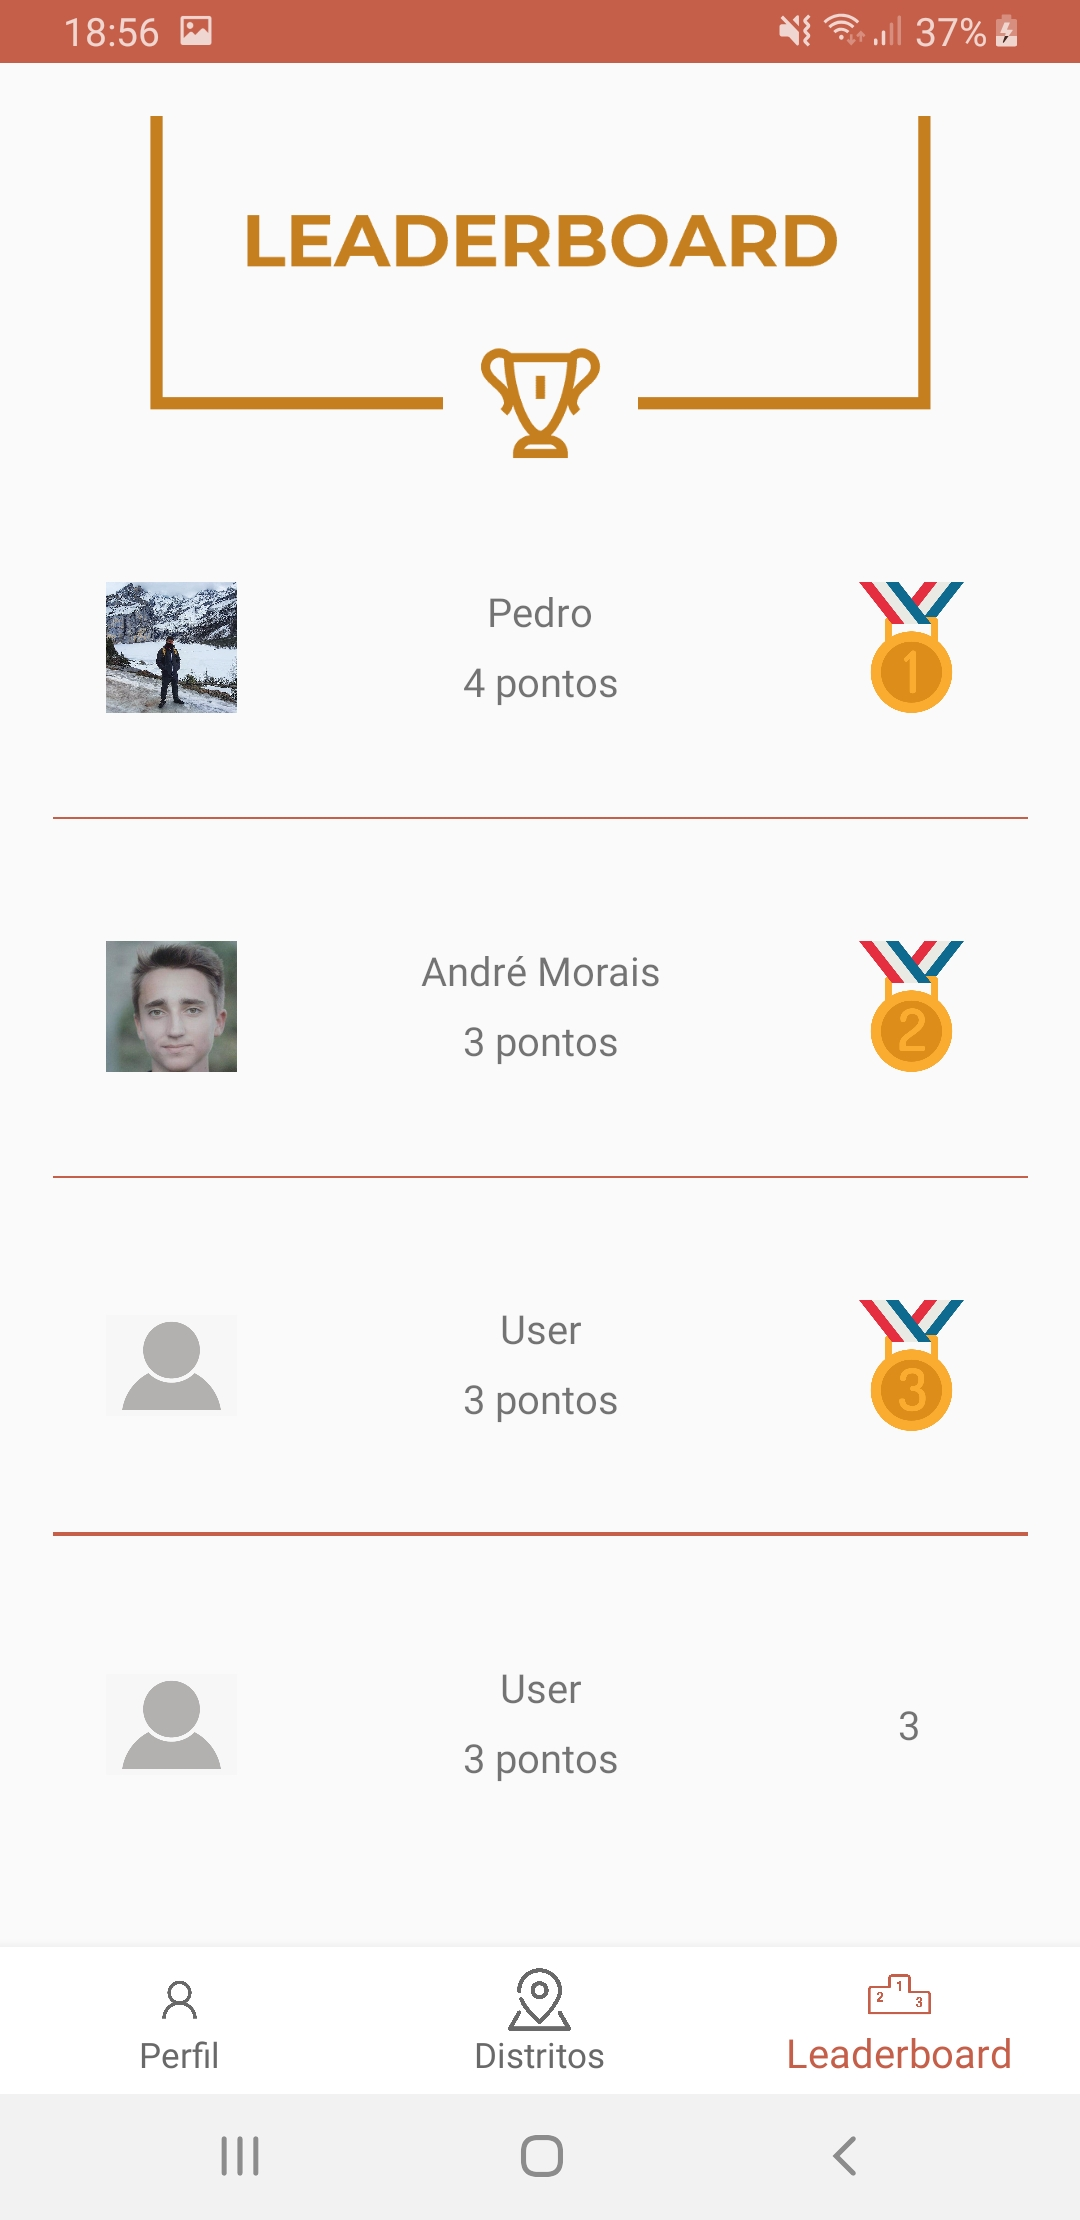
\includegraphics[width=0.5\linewidth]{images/leaderboard.jpg}
\caption{Tabela de classificações.}
\end{figure}
    
    \newpage
    
    \section{Base de Dados - Abordagem não relacional}
    \subsection{Justificação da utilização de um sistema NoSQL}
    Os sistemas de bases de dados relacionais assumem uma posição de predominância no mercado. Tal deve-se principalmente à eficácia do armazenamento dos dados estruturados. É importante referir que este tipo de sistemas preservam a consistência, integridade, isolamento dos dados e durabilidade. 
    
Contudo, surgiram problemas que conduziram ao aparecimento de sistemas de bases de dados não relacionais (NoSQL) que foram idealizados atendendo às lacunas que as bases de dados tradicionais demonstraram, com alta performance e capacidade de expansão. Estas, em vez de armazenarem os dados em tabelas, utilizam estruturas dependendo do tipo da base de dados, podendo estas serem, grafos, colunas, chave-valor e documentos.
    
    \subsection{MongoDB}
       MongoDB é uma base de dados NoSQL baseada em documentos. As suas características permitem que as aplicações modelem informações de modo mais natural, pois os dados podem ser agrupados em hierarquias complexas e continuarem a ser indexáveis e de fácil acesso.
   \par Para além disto:
    
    \begin{itemize}
        \item Permitem também uma maior escabilidade face às relacionais
        \item Sendo os requisitos da base de dados na sua maioria de natureza simples, o MongoDB terá uma eficiência maior apresentado os resultados em tempo inferior aos do MySQL.
        \item Sendo a base de dados multi-user, ou seja, utilizada por vários utilizadores ao mesmo tempo, o MongoDB apresenta também melhor performance no que toca ao acesso concorrente à base em questão.
    \end{itemize}

    \subsection{Implementação BD}
    Depois de um estudo às diferentes abordagens para a utilização de uma base de dados, ficou decidido que a utilização de um modelo não relacional, mais concretamente MongoDB, era o mais indicado.

Foi então necessário definir coleções para fundamentar a base de dados, nomeadamente:
\begin{itemize}
    \item Distritos
    \item Roteiros
    \item Users
\end{itemize}

De modo a que seja possível o bom funcionamento da aplicação, devem ser respeitados alguns campos para definir cada elemento presente nas coleções da base de dados.

  
    \subsubsection{Distrito}
    \begin{itemize}
    \item \texttt{string Nome} $\rightarrow$ Identifica o distrito pelo seu nome próprio, é necessário para apresentar o distrito na aplicação;
    \item \texttt{string ASCIIName} $\rightarrow$ Corresponde ao nome do distrito sem quaisquer caracter especial, tais como espaços, acentos e "ç". Importante para ser possível fazer chamadas à API devido aos pedidos HTTP;
    \item \texttt{int Pontos} $\rightarrow$ Número de pontos que o utilizador obtém sempre que visitar uma atração deste distrito;
    \item \texttt{string História} $\rightarrow$ Uma breve descrição sobre o distrito em si;
    \item \texttt{Lista de Cidades} $\rightarrow$ Lista com todas as cidades deste distrito. Estas cidades são objetos que guardam informações sobre as mesmas:
    \begin{itemize}
        \item \texttt{string Nome} $\rightarrow$ Identifica a cidade pelo seu nome próprio;
        \item \texttt{Lista de Atrações} $\rightarrow$ Indica todas as atrações da cidade:
        \begin{itemize}
            \item \texttt{string Nome} $\rightarrow$ Identifica a atração pelo seu nome próprio;
            \item \texttt{string Localidade} $\rightarrow$ Indica a local onde a atração está presente;
            \item \texttt{string História} $\rightarrow$ Breve descrição do local;
            \item \texttt{string Imagem} $\rightarrow$ URL representativo da imagem;
            \item \texttt{Lista Classificações} $\rightarrow$ Lista com todas as classificações feitas a esta atração:
            \begin{itemize}
            \item \texttt{string Email} $\rightarrow$ Email do utilizador que realizou a classificação;
            \item \texttt{string Classificação} $\rightarrow$ Número representativo da classificação feita pelo utilizador.
        \end{itemize}
        \end{itemize}
        \item \texttt{Lista de Restaurantes} $\rightarrow$ Indica todas os restaurantes da cidade:
        \begin{itemize}
            \item \texttt{string Nome} $\rightarrow$ Identifica o restaurante pelo seu nome próprio;
            \item \texttt{string Morada} $\rightarrow$ Tal como o nome indica, representa a morada do mesmo;
            \item \texttt{double Classificação} $\rightarrow$ Classificação do restaurante;
            \item \texttt{string Imagem} $\rightarrow$ URL representativo da imagem do restaurante.
        \end{itemize}
        \item \texttt{Lista de Hotéis} $\rightarrow$ Indica todas as hotéis da cidade:
        \begin{itemize}
            \item \texttt{string Nome} $\rightarrow$ Identifica o hotel pelo seu nome próprio;
            \item \texttt{string Morada} $\rightarrow$ Tal como o nome indica, representa a morada do mesmo;
            \item \texttt{int Classificação} $\rightarrow$ Classificação do restaurante;
            \item \texttt{string Imagem} $\rightarrow$ URL representativo da imagem do restaurante.
        \end{itemize}
    \end{itemize}
    \item \texttt{string Imagem} $\rightarrow$ URL da imagem para ser apresentada mais tarde
\end{itemize}
    
    \subsubsection{Utilizador}
    \begin{itemize}
    \item \texttt{string Nome} $\rightarrow$ Nome próprio do utilizador, apresentado no seu perfil;
    \item \texttt{string Email} $\rightarrow$ Email do utilizador, deve ser único;
    \item \texttt{string Distrito} $\rightarrow$ Distrito onde o utilizador vive;
    \item \texttt{string Cidade} $\rightarrow$ Cidade onde o utilizador vive;
    \item \texttt{string Password} $\rightarrow$ Password do utilizador, utilizada na sua autenticação. Deve ser segura e intransmissível;
    \item \texttt{string Imagem} $\rightarrow$ Imagem de perfil do utilizador, representada em base 64;
    \item \texttt{int Pontos} $\rightarrow$ Número de pontos conquistados pelo utilizador ao visitar diferentes atrações;
    \item \texttt{Lista de Publicações} $\rightarrow$ Representa o histórico do utilizador, que representa as atrações que o mesmo visitou:
    \begin{itemize}
        \item \texttt{string Distrito} $\rightarrow$ Indica o distrito onde fica a atração que o utilizador visitou;
        \item \texttt{string Atração} $\rightarrow$ Indica a atração visitada pelo utilizador;
        \item \texttt{string Imagem} $\rightarrow$ URL representativo da imagem da atração.
    \end{itemize}
\end{itemize}
    
    \subsubsection{Roteiro}
    \begin{itemize}
    \item \texttt{Lista de strings com Percurso} $\rightarrow$ Representa o percurso do roteiro, com a lista dos locais por onde ele passa;
    \item \texttt{string Descrição} $\rightarrow$ Breve descrição do roteiro;
    \item \texttt{string Imagem Roteiro} $\rightarrow$ URL com imagem apelativa do roteiro;
    \item \texttt{string Imagem Percurso} $\rightarrow$ URL com a imagem representativa do percurso do roteiro;
    \item \texttt{string Nome} $\rightarrow$ Nome indentificativo do roteiro;
    \item \texttt{string ASCII} $\rightarrow$ Nome do roteiro sem caracteres especiais, tais como espaços, acentos e "ç", de forma a ser possível realizar chamadas à API com o nome do roteiro. Deve ser único;
    \item \texttt{int Dist} $\rightarrow$ Indica a distância do percurso.
\end{itemize}

    \subsection{Acesso à Base de Dados}
    A aplicação desenvolvida pelo grupo deve estar funcional 24 horas durante 7 dias por semana, para isto, é necessário haver disponibilidade no acesso à base de dados durante todo este período de tempo. Por isso, houve necessidade de dar \textit{host} da base de dados na internet, para que fosse possível o acesso constante e remoto a toda a informação necessária para o funcionamento da aplicação.

A plataforma utilizada para manter a base de dados disponível todo o tempo foi \textbf{MongoDB Atlas}.
    
    \newpage
    
    \section{RestAPI - Comunicação entre cliente-servidor}
    
    \subsection{RestAPI}
    REST é um acrónimo para \textbf{RE}presentational \textbf{S}tate \textbf{T}ransfer e deve seguir 6 princípios fundamentais:
\begin{enumerate}
    \item \textbf{Client–server} - \textit{"By separating the user interface concerns from the data storage concerns, we improve the portability of the user interface across multiple platforms and improve scalability by simplifying the server components;"}
    \item \textbf{Stateless} - \textit{"Each request from client to server must contain all of the information necessary to understand the request, and cannot take advantage of any stored context on the server. Session state is therefore kept entirely on the client;"}
    \item \textbf{Cacheable} - \textit{"Cache constraints require that the data within a response to a request be implicitly or explicitly labeled as cacheable or non-cacheable. If a response is cacheable, then a client cache is given the right to reuse that response data for later, equivalent requests;"}
    \item \textbf{Uniform interface} - \textit{"By applying the software engineering principle of generality to the component interface, the overall system architecture is simplified and the visibility of interactions is improved. In order to obtain a uniform interface, multiple architectural constraints are needed to guide the behavior of components. REST is defined by four interface constraints: identification of resources; manipulation of resources through representations; self-descriptive messages; and, hypermedia as the engine of application state;"}
    \item \textbf{Layered system} - \textit{"The layered system style allows an architecture to be composed of hierarchical layers by constraining component behavior such that each component cannot “see” beyond the immediate layer with which they are interacting;"}
    \item \textbf{Code on demand (optional)} - \textit{"REST allows client functionality to be extended by downloading and executing code in the form of applets or scripts. This simplifies clients by reducing the number of features required to be pre-implemented;"}
\end{enumerate}
    
    \subsection{Implementação}
    Depois de um estudo às diferentes abordagens para a utilização de uma base de dados, ficou decidido que a utilização de um modelo não relacional, mais concretamente MongoDB, era o mais indicado.

Foi então necessário definir coleções para fundamentar a base de dados, nomeadamente:
\begin{itemize}
    \item Distritos
    \item Roteiros
    \item Users
\end{itemize}

De modo a que seja possível o bom funcionamento da aplicação, devem ser respeitados alguns campos para definir cada elemento presente nas coleções da base de dados.

    
    \subsection{Endpoits}
    A nossa RestAPI oferece os seguintes endpoints:

\begin{itemize}
    \item /api
    \begin{itemize}
        \item /distritos
        \begin{itemize}
            \item /nome
                \begin{itemize}
                    \item \textbf{GET} /:nomeASCII $\rightarrow$ Devolve o distrito com nomeASCII (representa o nome sem quaisquer caracter especial);
                    \item \textbf{PUT} /:nomeASCII $\rightarrow$ Atualiza o distrito com nomeASCII. Necessita dos dados do novo distrito;
                    \item \textbf{DELETE} /:nomeASCII $\rightarrow$ Elimina o distrito com nomeASCII.
                \end{itemize}
            \item \textbf{GET} / $\rightarrow$ Devolve todos os distritos presentes na base de dados;
            \item \textbf{GET} /:id $\rightarrow$ Devolve o distrito com id enviado como parametro;
            \item \textbf{POST} / $\rightarrow$ Insere um distrito na base de dados;
            \item \textbf{PUT} /:id $\rightarrow$ Atualiza um distrito consoante o seu id;
            \item \textbf{DELETE} / $\rightarrow$ Elimina um distrito da base de dados. Necessita dos dados do distrito a eliminar;
            \item \textbf{DELETE} /:id $\rightarrow$ Elimina um distrito da base de dados consoante o seu id.
        \end{itemize}
        \item /users
        \begin{itemize}
            \item /email
                \begin{itemize}
                    \item \textbf{GET} /:email $\rightarrow$ Devolve o utilizador com email enviado como parametro;
                    \item \textbf{PUT} /:email $\rightarrow$ Atualiza o utilizador consoante o seu email;
                    \item \textbf{DELETE} /:email $\rightarrow$ Elimina o utilizador consoante o seu email.
                \end{itemize}
            \item \textbf{GET} / $\rightarrow$ Devolve todos os utilizadores presentes na base de dados;
            \item \textbf{GET} /:id $\rightarrow$ Devolve o utilizador consoante o seu id;
            \item \textbf{POST} / $\rightarrow$ Insere um utilizador na base de dados;
            \item \textbf{PUT} /:id $\rightarrow$ Atualiza um utilizador consoante o seu id;
            \item \textbf{DELETE} / $\rightarrow$ Elimina um utilizador da base de dados;
            \item \textbf{DELETE} /:id $\rightarrow$ Elimina o utilizador da base de dados consoante o seu id.
        \end{itemize}
        \item /roteiros
        \begin{itemize}
            \item /nome
                \begin{itemize}
                    \item \textbf{GET} /:nomeASCII $\rightarrow$ Devolve o roteiro consoante o seu nomeASCII;
                    \item \textbf{PUT} /:nomeASCII $\rightarrow$ Atualiza o roteiro consoante o seu nomeASCII;
                    \item \textbf{DELETE} /:nomeASCII $\rightarrow$ Elimina o roteiro consoante o seu nomeASCII.
                \end{itemize}
            \item \textbf{GET} / $\rightarrow$ Devolve todos os roteiros presentes na base de dados;
            \item \textbf{GET} /:id $\rightarrow$ Devolve um roteiro consoante o id do mesmo;
            \item \textbf{POST} / $\rightarrow$ Insere um roteiro na base de dados;
            \item \textbf{PUT} /:id $\rightarrow$ Atualiza um roteiro consoante o seu id;
            \item \textbf{DELETE} / $\rightarrow$ Elimina um roteiro da base de dados;
            \item \textbf{DELETE} /:id $\rightarrow$ Elimina um roteiro consoante o seu id.
        \end{itemize}
    \end{itemize}
\end{itemize}
    
    \subsection{Demonstração}
    \begin{figure}[H]
\centering
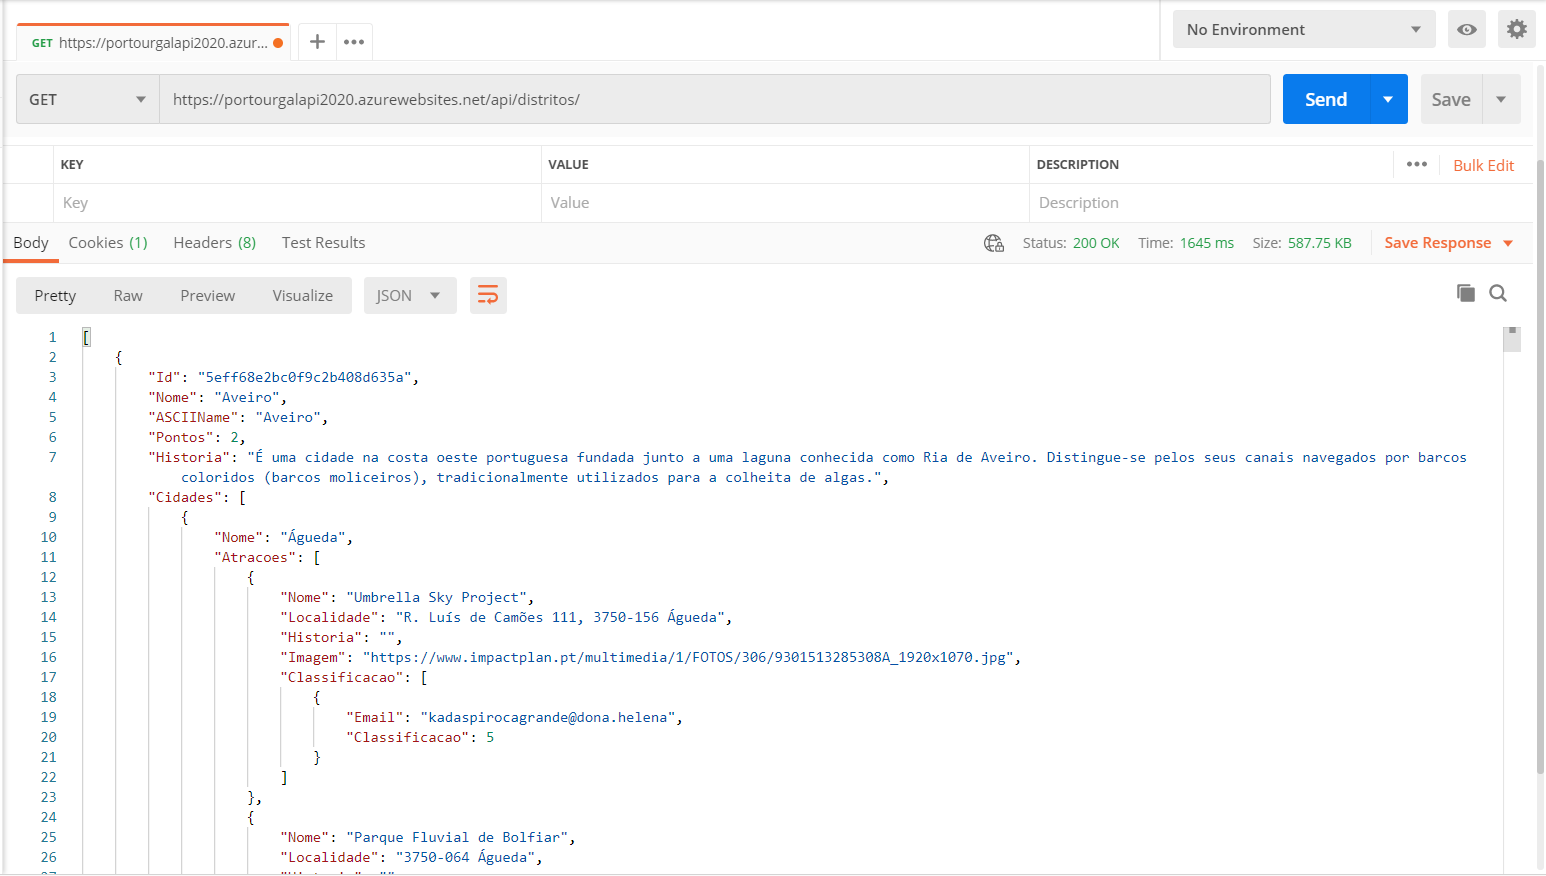
\includegraphics[width=\linewidth]{images/api_distritos.png}
\caption{GET /distritos.}
\end{figure}

\begin{figure}[H]
\centering
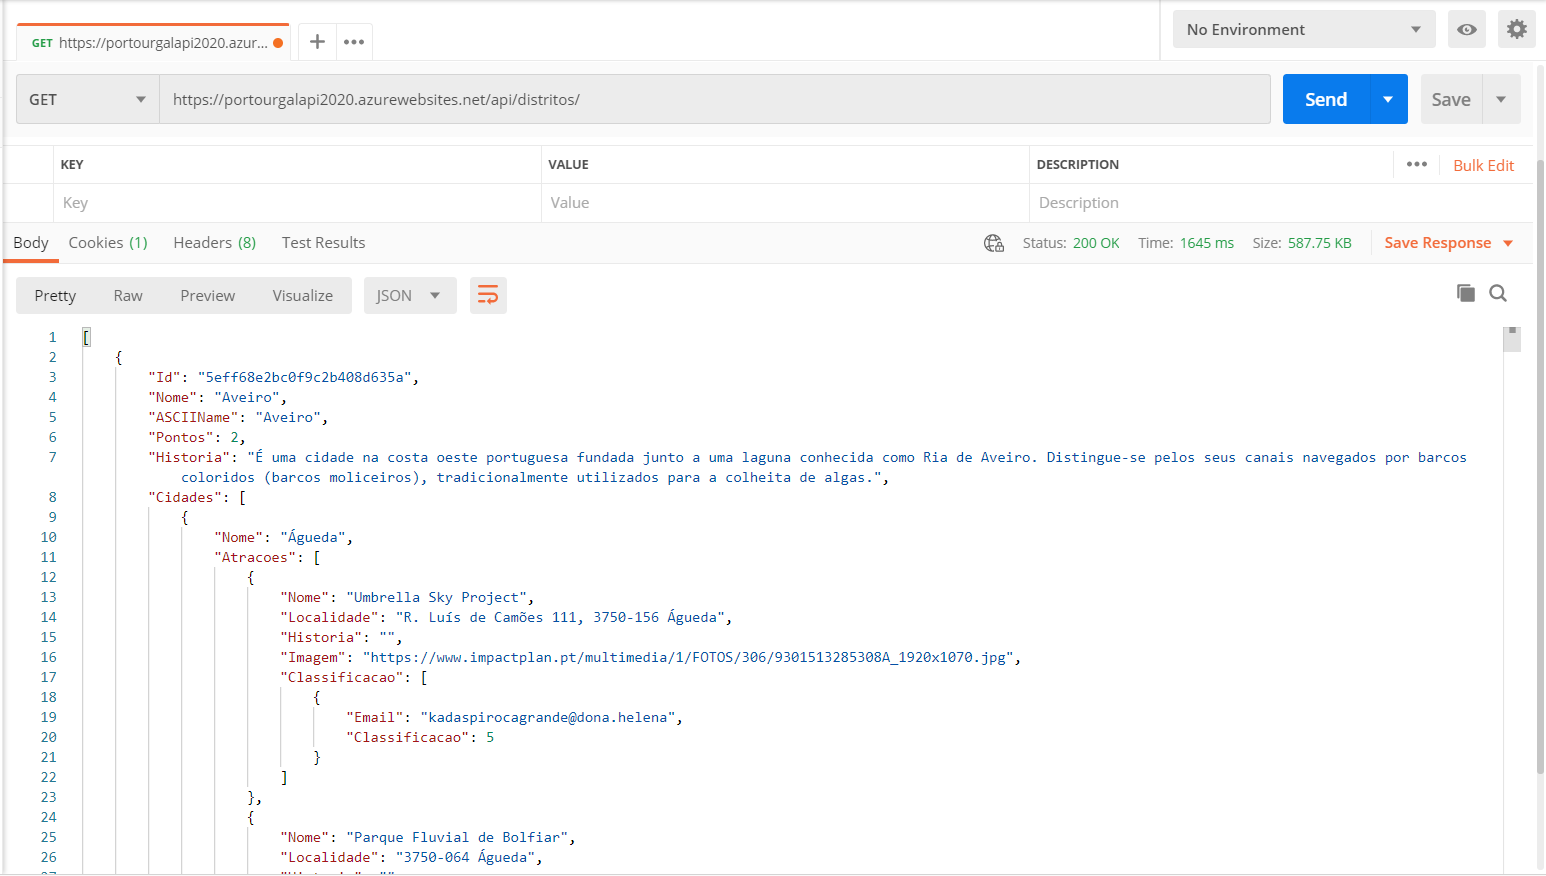
\includegraphics[width=\linewidth]{images/api_distritos.png}
\caption{GET /distritos/nome/:nomeASCII.}
\end{figure}

\begin{figure}[H]
\centering
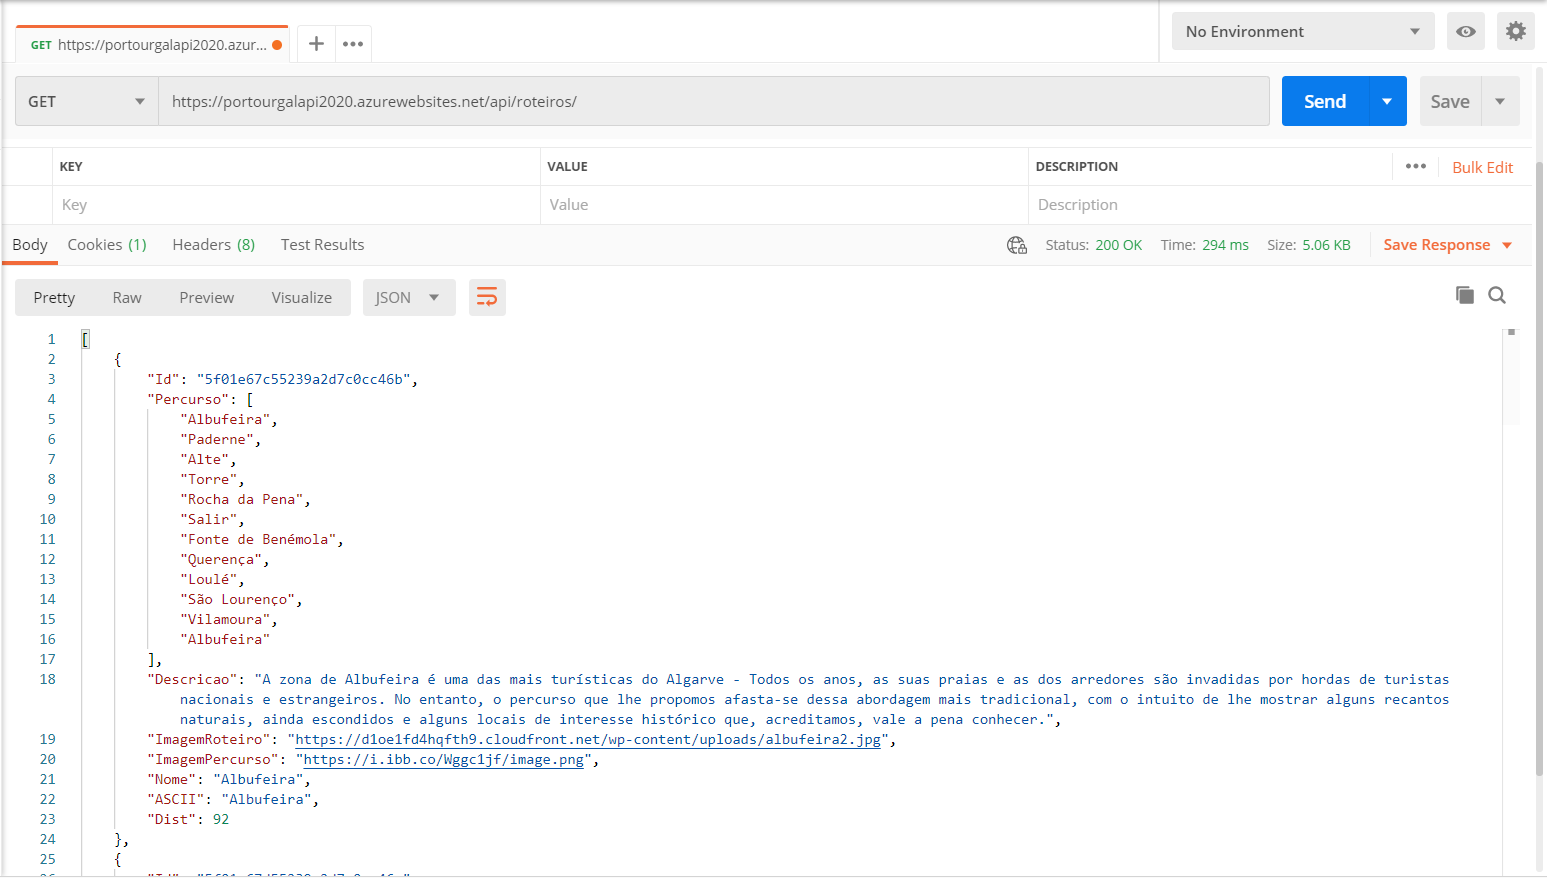
\includegraphics[width=\linewidth]{images/api_roteiro.png}
\caption{GET /roteiros.}
\end{figure}

\begin{figure}[H]
\centering
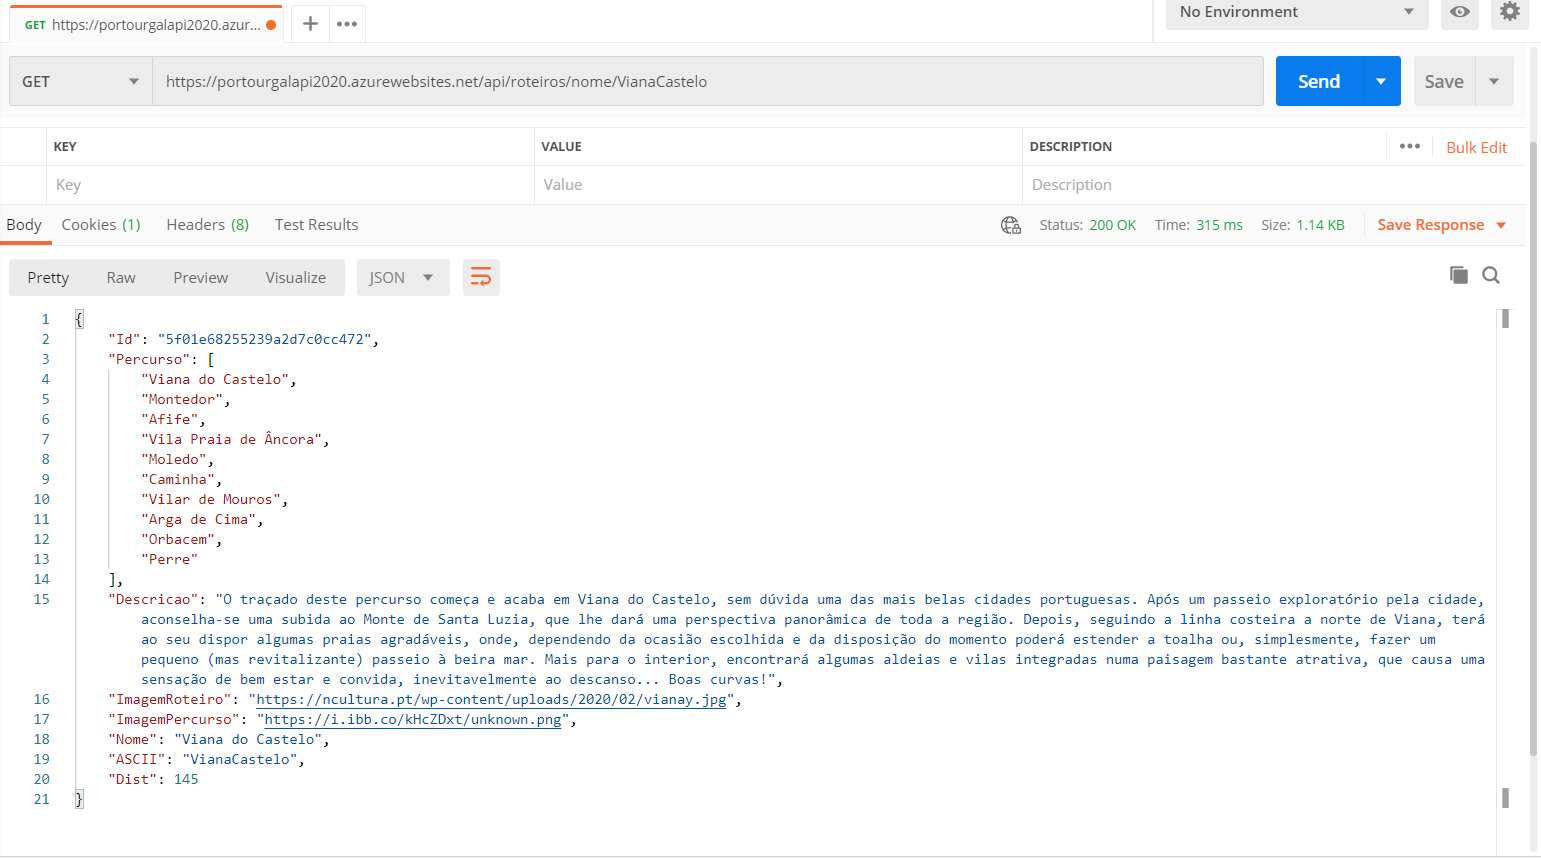
\includegraphics[width=\linewidth]{images/api_roteiroviana.png}
\caption{GET /roteiros/nome/:nomeASCII.}
\end{figure}

\begin{figure}[H]
\centering
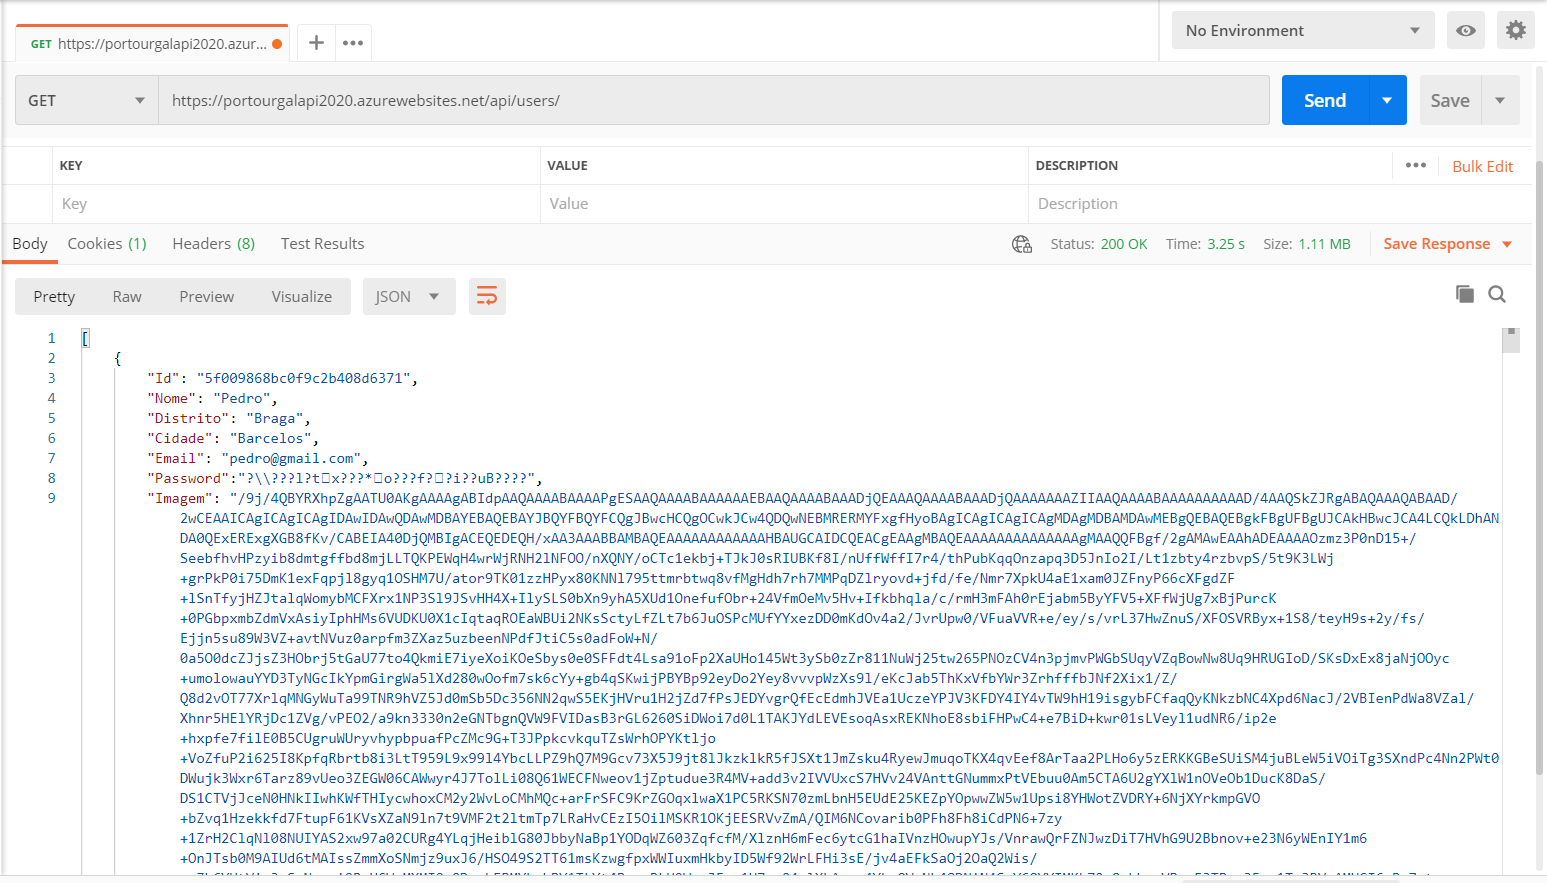
\includegraphics[width=\linewidth]{images/api_user.png}
\caption{GET /users.}
\end{figure}

\begin{figure}[H]
\centering
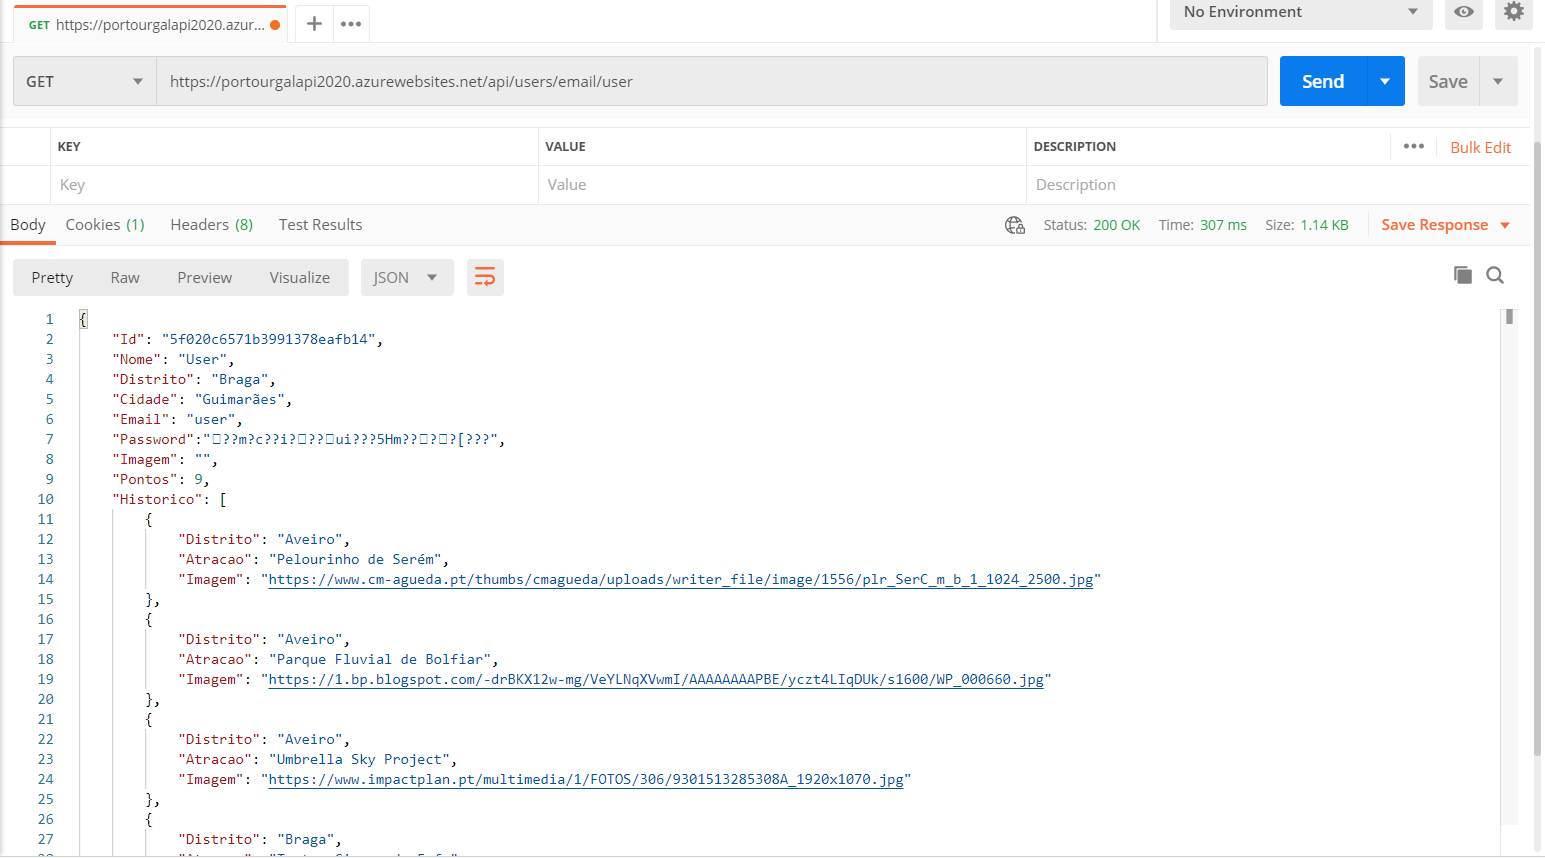
\includegraphics[width=\linewidth]{images/api_userluk.png}
\caption{GET /users/nome/:nomeASCII.}
\end{figure}
    
    \subsection{API externa}
    Tal como previsto na idealização do projeto, foi utilizada uma API externa que fornece dados sobre a meteorologia em tempo real. Esta API foi utilizada para apresentar ao cliente o estado do tempo, bem como a temperatura, nas atrações de um determinado distrito.

A API escolhida foi \textbf{Open Weather Map API}, que mantém a sua documentação em \url{http://openweathermap.org/current}.

Na aplicação desenvolvida fora utilizada duas chamada à API externa:

\begin{enumerate}
    \item \textbf{weather?q=[Distrito],PT\&lang=pt\&units=metric\&appid=[API Key]} - Retorna todo o tipo de informações acerca da meteorologia no local. Os campos utilizados foram a decrição, a temperatura, e o código do icon;
    \item \textbf{/img/wn/[Código Icon].png} - Devolve a imagem representativa do código de icon devolvido pela chamada anterior.
\end{enumerate}

    
    \newpage
    
    \section{Cliente - Servidor - Base de Dados}
    Introdução
    
    \section{Segurança}
    Introdução
    
    \subsection{Implementação}
    Depois de um estudo às diferentes abordagens para a utilização de uma base de dados, ficou decidido que a utilização de um modelo não relacional, mais concretamente MongoDB, era o mais indicado.

Foi então necessário definir coleções para fundamentar a base de dados, nomeadamente:
\begin{itemize}
    \item Distritos
    \item Roteiros
    \item Users
\end{itemize}

De modo a que seja possível o bom funcionamento da aplicação, devem ser respeitados alguns campos para definir cada elemento presente nas coleções da base de dados.

    
    \newpage
    
    \section{Administração do Sistema}
    Os sistemas de bases de dados relacionais assumem uma posição de predominância no mercado. Tal deve-se principalmente à eficácia do armazenamento dos dados estruturados. É importante referir que este tipo de sistemas preservam a consistência, integridade, isolamento dos dados e durabilidade. 
    
Contudo, surgiram problemas que conduziram ao aparecimento de sistemas de bases de dados não relacionais (NoSQL) que foram idealizados atendendo às lacunas que as bases de dados tradicionais demonstraram, com alta performance e capacidade de expansão. Estas, em vez de armazenarem os dados em tabelas, utilizam estruturas dependendo do tipo da base de dados, podendo estas serem, grafos, colunas, chave-valor e documentos.
    
    \subsection{Demonstração}
    \begin{figure}[H]
\centering
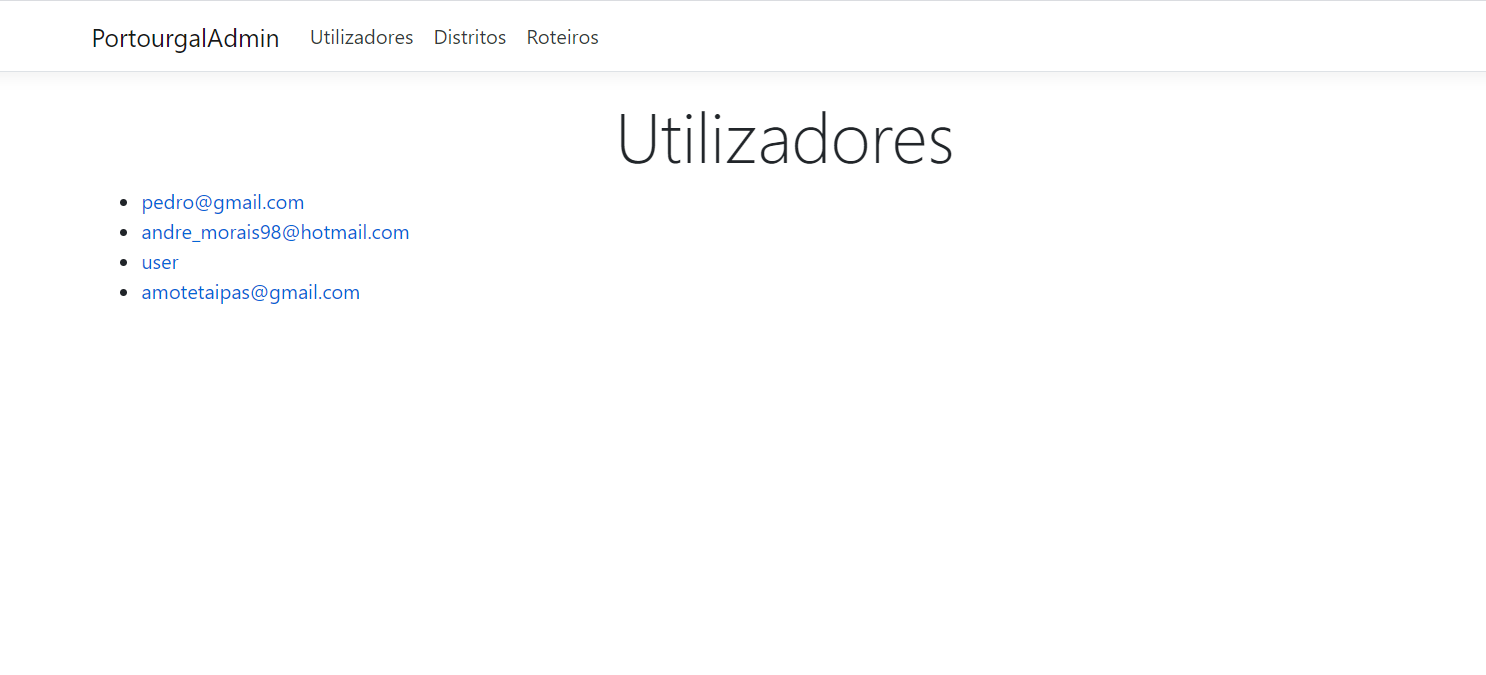
\includegraphics[width=0.7\linewidth]{images/site_utilizadores.png}
\caption{Visualização de todos utilizadores.}
\end{figure}

\begin{figure}[H]
\centering
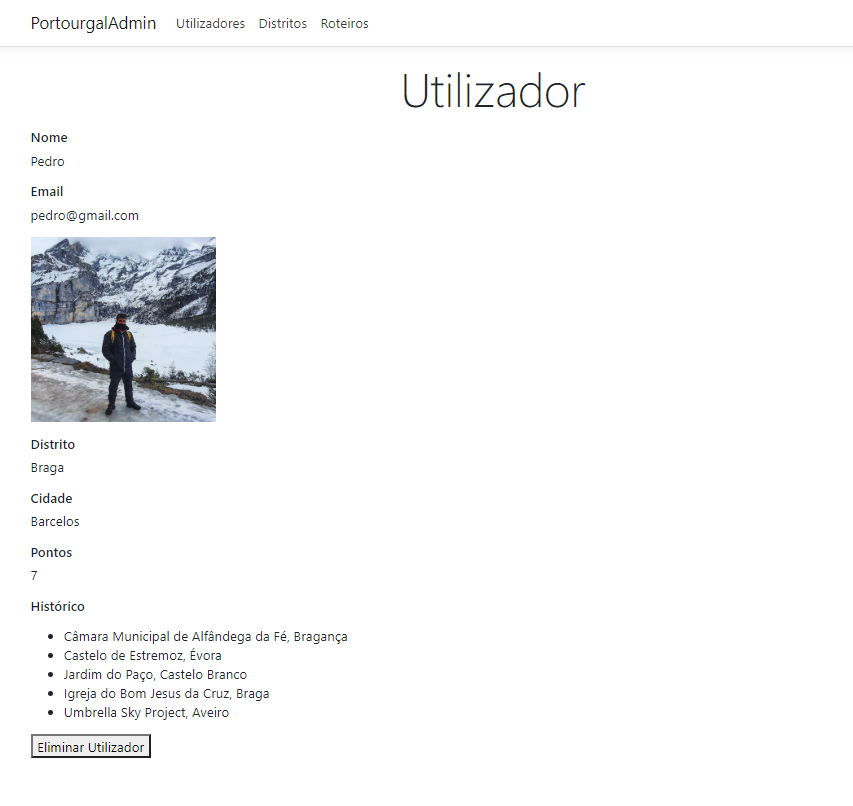
\includegraphics[width=0.7\linewidth]{images/site_utilizador.png}
\caption{Visualização de um utilizador.}
\end{figure}

\begin{figure}[H]
\centering
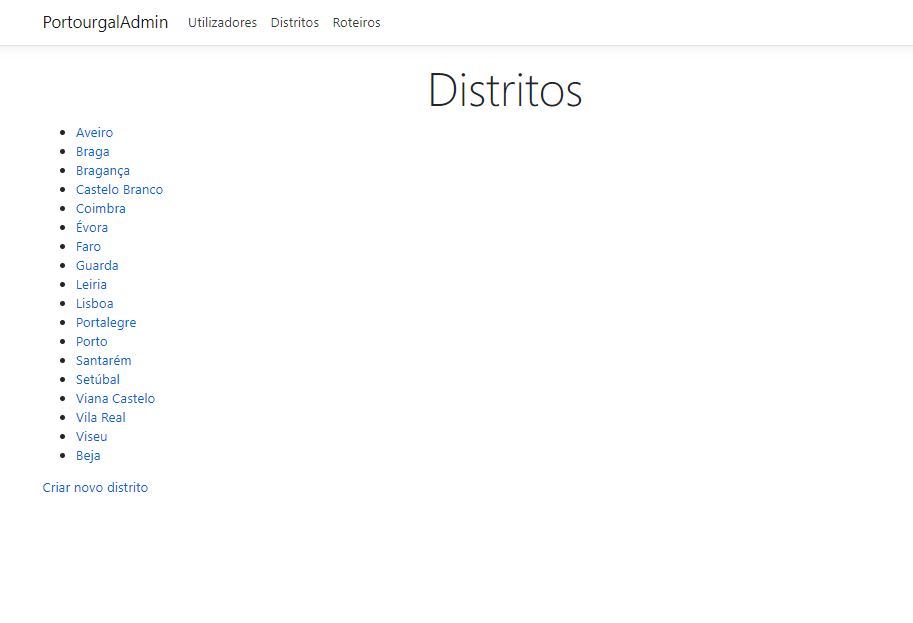
\includegraphics[width=0.7\linewidth]{images/site_distritos.png}
\caption{Visualização de todos os distritos.}
\end{figure}

\begin{figure}[H]
\centering
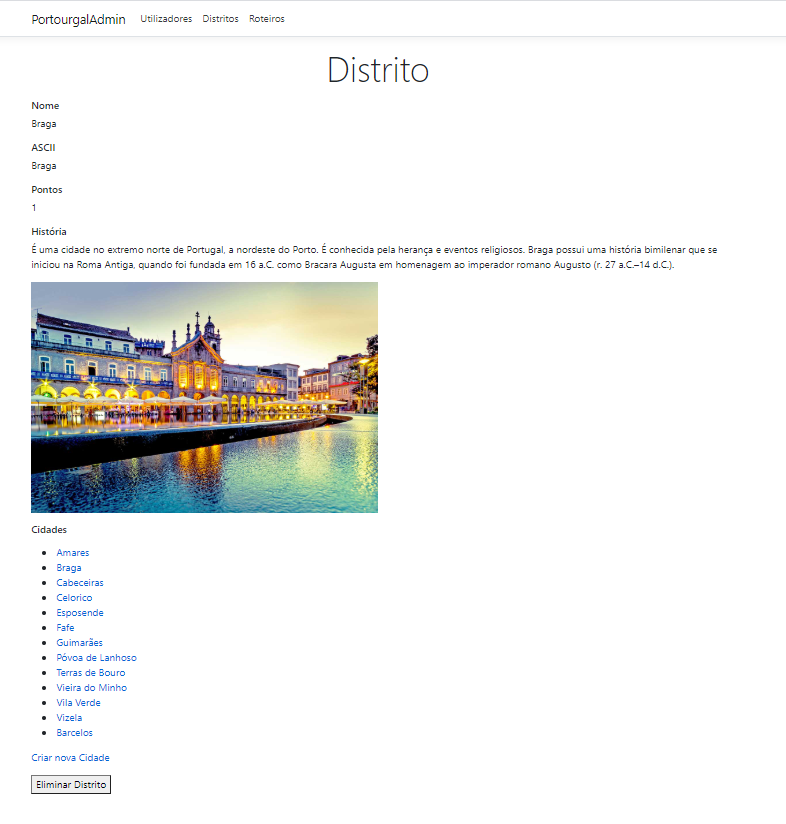
\includegraphics[width=0.7\linewidth]{images/site_distrito.png}
\caption{Visualização de um distrito, contendo todas as cidades.}
\end{figure}

\begin{figure}[H]
\centering
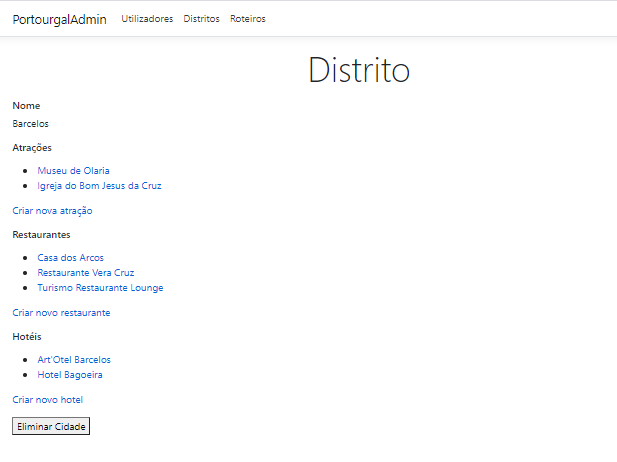
\includegraphics[width=0.7\linewidth]{images/site_cidade.png}
\caption{Visualização de uma cidade, contendo todas as atrações, restaurantes e hotéis.}
\end{figure}

\begin{figure}[H]
\centering
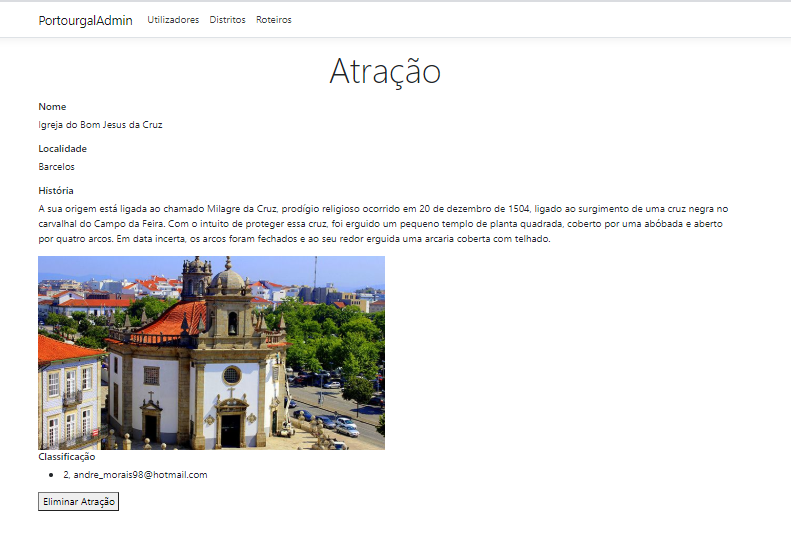
\includegraphics[width=0.7\linewidth]{images/site_atracao.png}
\caption{Visualização de uma atração.}
\end{figure}

\begin{figure}[H]
\centering
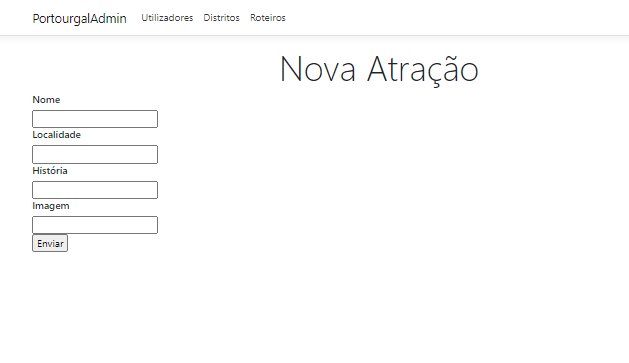
\includegraphics[width=0.7\linewidth]{images/site_nova_atracao.png}
\caption{Criação de uma nova atração.}
\end{figure}

\begin{figure}[H]
\centering
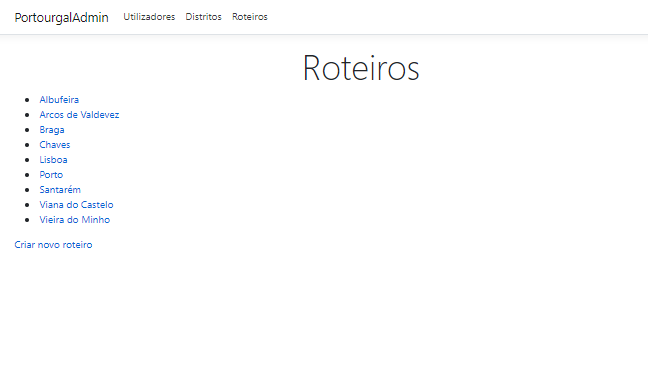
\includegraphics[width=0.7\linewidth]{images/site_roteiros.png}
\caption{Visualização de todos os roteiros.}
\end{figure}

\begin{figure}[H]
\centering
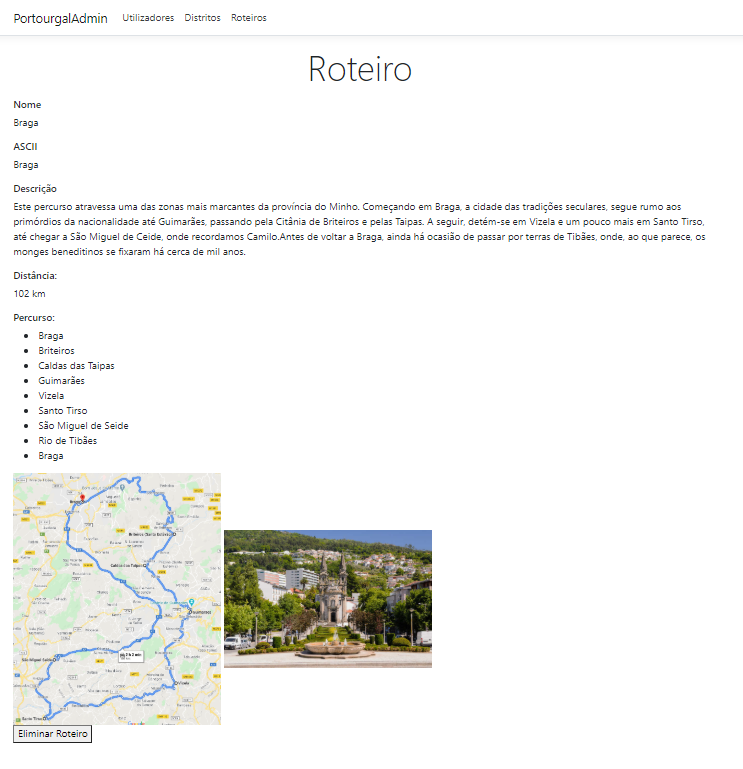
\includegraphics[width=0.7\linewidth]{images/site_roteiro.png}
\caption{Visualização de um roteiro.}
\end{figure}

    
    \section{Identificação dos recursos utilizados}
    Ao nível do desenvolvimento da aplicação foi necessário dispor de recursos humanos, de hardware e de software.
Os recursos humanos englobam os trabalhadores envolvidos no projeto e as horas dedicadas neste mesmo. Quanto aos recursos de hardware indispensáveis para o desenvolvimento da “PORTOURGAL” foram as máquinas pessoais dos elementos do grupo.
Para além destes aspetos, foram utilizadas as seguintes ferramentas no decorrer do desenvolvimento do projeto:
\begin{itemize}
    \item \textbf{Visual Paradigm} – plataforma usada para a modelação do projeto;
    \item \textbf{Latex} - plataforma usada para a escrita do relatório;
    \item \textbf{MongoDB Atlas} - plataforma usada para a persistência de dados;
    \item \textbf{Microsoft Visual Studio} - ambiente de desenvolvimento das aplicações .NET;
    \item \textbf{Microsoft .NET C#} - plataforma usada para a codificação da aplicação;
    \item \textbf{Adobex XD} - ferramenta de design para a construção dos mockups;
    \item \textbf{Postman} - plataforma usada para facilitar as chamadas à API;
    \item \textbf{Weather API} - API para obter o clima;
    \item \textbf{Microsoft Azure} - plataforma usada para dar host à API;
    \item \textbf{Google & Booking} - usado para o povoamento da Base de Dados.
\end{itemize}
    
    \newpage

	% CHAPTER - Conclusion/Future Work --------------
	\chapter{Conclusion}
	Ao longo da realização deste trabalho prático, o grupo foi-se deparando com as diversas fases na produção de aplicações, esforçando-se para ultrapassar todas as dificuldades que delas advêm.

Para a primeira fase – a \textbf{Fundamentação} – foram reunidos os pilares fundamentais do projeto: Contextualizou-se o problema, definiram-se os objetivos a cumprir, estudou-se a viabilidade, complexidade e utilidade do sistema a desenvolver, e de seguida listamos os recursos que serão necessários para as subsequentes fases. Esta fase é fulcral pois catalisam desde já a criação de um caminho para a compreensão e modelação com sucesso do sistema de Software.

O plano de desenvolvimento, que foi apresentado na forma de um Diagram de Gantt, foi uma ajuda preciosa pois permitiu organizar e quantificar o número de horas de trabalho necessárias para o desenvolvimento da peça de software proposta.

Na segunda fase – a \textbf{Especificação} – procedeu-se à modelação do projeto assente nos princípios ajustados na fase anterior. Primeiramente foram identificados os requisitos não funcionais e funcionais. De seguida, elaboraram-se alguns diagramas UML considerados relevantes para a compreensão do sistema a ser desenvolvido, tais como: 
\begin{itemize}
    \item Modelo de Domínio
    \item Diagrama Use Cases
    \item Diagrama de Classes
\end{itemize}

O Modelo de Domínio é claro e conciso. Esta propriedade, assim como a identificação correta dos diferentes papéis dos relacionamentos entre as entidades, vão de encontro aos objetivos que traçamos no começo da concessão do projeto. Relativamente ao Diagrama de Use Cases, permitiu capturar requisitos funcionais, fornecendo assim uma notação diagramática que permite modelar o contexto geral do sistema. O Diagrama de Classes permite ilustrar as classes e o relacionamento entre as mesmas, daí ser tão importante implementar.

Para lá da simplificação do problema, adicionalmente, estes modelos, contribuíram para obtermos uma ideia final clara e objetiva de todo o sistema de software implementado.

Estruturou-se a base de dados sólida e esboçaram-se mockups, idealizando a interface e camadas de apresentação do sistema.

Para a terceira e última fase deste projeto – a \textbf{Implementação} –, debruçámo-nos sobre a sobre a produção do software. Tendo por base todo o trabalho desenvolvido referente à modelação, criou-se uma aplicação Web que considerámos cumprir as diretrizes mais relevantes estabelecidas pelo cliente.

O grupo deparou-se com uma linguagem de programação que não tinha sido trabalhada até ao momento, ferramentas de produção de software desconhecidas e um paradigma de desenvolvimento novo. Todos estes fatores contribuíram para que o planeamento não fosse cumprido como tinha sido idealizado na primeira fase de projeto, levando a que este fosse ocasionalmente alterado. Apesar do grupo perceber que deveria ter seguido à risca o plano idealizado no início do projeto (o que não foi possível por não termos experiência com este tipo de aplicações e linguagem), também soube ter um lado mais prático e pro-ativo, por forma a ter um produto final (inacabado) para entregar ao cliente.

Assim sendo, – e apesar dos obstáculos encontrados - o grupo pensa que o seu trabalho foi positivo. O produto final é funcional, satisfaz todos os Use Cases feitos e, acima de tudo, é flexível e utilizável o que sugere que trará bastante entusiasmo aos futuros utilizadores da aplicação.

			
	\bookmarksetup{startatroot} % Ends last part.
	\addtocontents{toc}{\bigskip} % Making the table of contents look good.
	%\cleardoublepage

	%- Bibliography (needs bibtex) -%
	%\bibliography{dissertation}

	% Index of terms (needs  makeindex) -------------
	%\printindex
	
	
	% APPENDIX --------------------------------------
	%\umappendix{Appendix}
	
	% Add appendix chapters
	%\chapter{Support material}
	%Auxiliary results which are not main-stream; or

	%\chapter{Details of results}
	%Details of results whose length would compromise readability of main text; or

	%\chapter{Listings}
	%Specifications and Code Listings: should this be the case; or

	%\chapter{Tooling}
	%Tooling: Should this be the case.

	%Anyone using \Latex\ should consider having a look at \TUG,
	%the \tug{\TeX\ Users Group}


	% Back Cover -------------------------------------------
	%\umbackcover{
	%NB: place here information about funding, FCT project, etc in which the work is framed. Leave empty otherwise.
	%}


\end{document}
